\documentclass[10pt]{article}

\usepackage{amsmath}
\usepackage{mathtools}
\usepackage{graphicx}
\usepackage{amssymb}
\graphicspath{ {./} }
\usepackage{float}
\usepackage{wrapfig}
\usepackage[none]{hyphenat}
\numberwithin{equation}{section}
\numberwithin{figure}{section}
\numberwithin{table}{section}
\usepackage{mdframed}

\usepackage[romanian]{babel}
\usepackage{combelow}
\useshorthands{'}
\useshorthands{;}
\defineshorthand{'s}{\cb{s}}
\defineshorthand{'t}{\cb{t}}
\defineshorthand{'S}{\cb{S}}
\defineshorthand{'T}{\cb{T}}
\defineshorthand{;a}{\u{a}}
\defineshorthand{;A}{\u{A}}
\defineshorthand{'a}{\^{a}}
\defineshorthand{'A}{\^{A}}
\defineshorthand{'i}{\^{i}}
\defineshorthand{'I}{\^{I}}


\title{Aplica'tii ale re'telelor neuro-fuzzy 'in estimarea costului dezvolt;arii software}
\date{20 august 2017}
\author{Madar Nicu'sor-Florin}

\begin{document}
\pagenumbering{gobble}
\newpage
\thispagestyle{empty}
\mbox{}
\newpage

\begin{center}
\large
UNIVERSITATEA DIN BUCURE'STI\\
FACULTATEA DE MATEMATIC;A 'SI INFORMATIC;A\\
\end{center}

\vspace{1.5cm}

\begin{center}
\textbf{
{\LARGE Lucrare de licen't;a\\
\medskip
Aplica'tii ale re'telelor neuro-fuzzy\\
 'in estimarea costului dezvolt;arii software\\}}
\end{center}

\vspace{7cm}

\begin{minipage}{\textwidth}
\Large
Coordonator 'stiin'tific,\\
Lect. dr. 'Suter Florentina
\begin{flushright}
\Large
Student,\\
Madar Nicu'sor-Florin
\end{flushright}
\end{minipage}

\vspace{2cm}
\begin{center}
\Large
Bucure'sti\\
2017
\end{center}






\newpage

\newpage
\thispagestyle{empty}
\mbox{}
\newpage

\tableofcontents
\newpage

\pagenumbering{arabic}

\section{Introducere}

\paragraph{}

Prin lucrarea de fa't;a dorim s;a prezent;am un studiu asupra re'telelor neuro-fuzzy aplicate peste modelul COCOMO (\textit{Constructive Cost Model}), astfel 'inc'at s;a se poat;a ob'tine o estimare a dezvolt;arii unui proiect software plec;and de la factorii de cost 'si dimensiunea sa. Metoda prezentat;a este centrat;a pe re'telele ANFIS (\textit{Adaptive neuro-fuzzy inference system}), un tip de re'tele neuronale relativ nou, articolul 'in care au fost definite fiind publicat 'in 1993.

\par
F;ar;a a intra in detalii deocamdat;a, re'telele neuro-fuzzy, datorit;a faptului c;a sunt alc;atuite dintr-o re'tea neuronal;a 'si un sistem de inferen't;a fuzzy, ofer;a at'at puterea de 'inv;a'tare a re'telelor neuronale clasice, c'at 'si flexibilitatea logicii fuzzy de a lucra cu date incerte \cite{anfis}. Deoarece, 'in mod inerent, orice estimare este supus;a subiectivit;a'tii, 'si nici modelul COCOMO nu ofer;a o metod;a riguroas;a pentru alegerea factorilor de cost, este de 'in'teles c;a o predic'tie de cost pleac;a de la premisa c;a datele de intrare sunt \textit{subiective}, i.e. au un oarecare grad de incertitudine. Astfel, problema de fa't;a devine un candidat bun pentru o re'tea neuro-fuzzy. 

\par
Modelul COCOMO dateaz;a din 1981 'in cartea lui Barry W. Boehm \textit{"Software Engineering Economics"} \cite{boehm}, fiind un model pentru estimarea efortului, costului si gestion;arii timpului de dezvoltare al proiectelor software. Acesta este o combina'tie de trei modele cu niveluri diferite de detalii 'si complexitate:
\begin{itemize}
\item Basic: ofer;a o estimare rapid;a;\ se preteaz;a 'in stagiile precare ale dezvolt;arii
\item Intermediate: estim;arile devin mai precise, sunt necesare caracteristici ale proiectului 'si un stagiu mai matur de dezvoltare
\item Advanced: cel mai detaliat dintre toate trei, necesit;a cea mai mult;a informa'tie
\end{itemize}
Lucrarea trateaz;a nivelul \textit{Intermediate} al COCOMO, acesta oferind un echilibru bun 'intre datele de intrare (15 factori de cost 'si o estimare numeric;a a dimensiunii proiectului 'in linii de cod surs;a) 'si acurate'tea estim;arii efortului 'in \textit{man-months}. 

\par
'In afara sec'tiunilor de introducere, lucrarea este 'imp;ar'tit;a 'in dou;a p;ar'ti. 'In prima parte vom prezenta aspectele teoretice pentru a fundamenta 'si analiza tehnicile folosite 'in construirea 'si antrenarea unei re'tele neuro-fuzzy peste modelul COCOMO. 'In cea de-a doua parte lucrarea va prezenta rezultatele ob'tinute, f;ac'and 'si o compara'tie sumar;a cu rezultatele ce au fost ob'tinute deja 'in domeniu.

\par
Lucrarea se 'incheie printr-o compara'tie cu o re'tea neuronal;a clasic;a, pentru a expune diferen'tele fa't;a de un model conven'tional 'si bine stabilit 'in acest domeniu pentru problemele de \textit{fitting}.

\par
\section{Prezentarea Domeniului}

\paragraph{}

\par
Exist;a o mul'time de articole scrise at'at pe tema estim;arii costurilor de dezvoltare folosind COCOMO, c'at 'si pentru estimarea acestora folosind tehnici neuro-fuzzy. Vom prezenta 'in continuare, 'in mod sumar, dou;a articole pentru a oferi lucr;arii de fa't;a un context 'si o 'incadrare 'in domeniu.
\par
Primul articol pe care 'il vom prezenta este "COCOMO Estimates Using Neural Networks" \cite{cocomoneuralnets}, o lucrare ce prezint;a rezultatele experimentale ale estim;arii modelului COCOMO folosind o re'tea neuronal;a cu trei straturi. Kaushik et al. prezint;a o metodologie de 'inv;a'tare pe setul de date COCOMO disponibil public, evalu'and performan'ta arhitecturii folosind criteriul de evaluare MRE (\textit{Magnitude of Relative Error}). Autorii men'tioneaz;a c;a urm;aresc ob'tinerea unei re'tele cu un num;ar c'at mai mic de straturi de perceptroni 'si de noduri, astfel 'inc'at performan'tele re'telei s;a fie c'at mai bune, dar complexitatea acesteia, 'si, implicit, timpul necesar pentru antrenare s;a fie minimizat.
\par
Av'and ponderile $W_{i}, i = \overline{1, 17}$ ini'tializate cu 1, rata de 'inv;a'tare $\alpha = 0.001$ 'si biasul $b = 1$, algoritmul propus este prezentat 'in 'sapte pa'si:
\begin{enumerate}
\item Execut;a pa'sii 2-7 p'an;a c'and condi'tia de oprire este fals;a.
\item Execut;a pa'sii 3-6 pentru fiecare pereche de antrenare.
\item Stratul de intrare prime'ste semnalul de intrare 'si 'il trimite c;atre stratul ascuns prin aplicarea func'tiilor identitate de activare pentru toate nodurile de intrare $v_{i}, i = \overline{1, 17}$.
\item Fiecare nod ascuns 'i'si 'insumeaz;a semnalele de intrare ponderate pentru a calcula ie'sirea re'telei dup;a formula:
\begin{equation} y_{in j} = b_{j} + \displaystyle\sum_{i=1}^{17} v_{i}W_{ij} \end{equation}
Func'tia de activare a perceptronului $f(y_{in})$ este aplicat;a pentru fiecare nod, unde 
\begin{equation}
f(y_{in}) = \begin{cases}
		1  & \quad \text{dac;a } y_{in} > \theta \\
		0  & \quad \text{dac;a } -\theta \leq y_{in} \leq \theta\\
		-1 & \quad \text{dac;a } y_{in} < -\theta
\end{cases}
\end{equation}
este func'tia de activare, cu $\theta$ fiind o valoare de prag.
\item Calculeaz;a ie'sirile (i.e. efortul) pe stratul de ie'sire folosind aceea'si procedur;a ca 'in pasul 4 consider'and toate ponderile pentru $j = \overline{1, 5}$ ca fiind $1$.
\item Compar;a efortul real cu cel estimat;\ dac;a diferen'ta este 'in limitele acceptate atunci rezultatul este acceptat, altfel ponderile sunt actualizate dup;a:
\begin{equation}
W_{i}(nou) = W_{i}(vechi) + \alpha \cdot intrare(i)
\end{equation}
\item Verific;a dac;a rezultatele se supun condi'tiei de operire i.e. dac;a nu exist;a nicio schimbare 'in ponderi atunci opre'ste procesul de antrenare, altfel reporne'ste de la pasul 2.
\end{enumerate}

Folosind metoda prezentat;a, autorii 'incheie articolul ajung'and la concluzia c;a o re'tea neuronal;a ofer;a o acurate'te acceptabil;a pentru predic'tie asupra datelor din setul de date COCOMO '81., 'incerc'and s;a 'il modeleze folosind o re'tea cu un num;ar de noduri c'at mai mic, pentru a p;astra performan'ta.
\par
Al doilea articol pe care 'il vom prezenta este "Software Cost Estimation using Adaptive Neuro Fuzzy Inference System" \cite{anfiscost}, o lucrare ce folose'ste un model de re'tele neuro-fuzzy pentru a prezenta rezultate experimentale ale estim;arii modelului COCOMO. Autorii prezint'a o metod;a ce implic;a normalizarea datelor de intrare 'inainte ca acestea s;a fie prezentate re'telei, ei suger'and normalizarea min-max. Normalizarea min-max este definit;a ca:
\begin{equation} 
x' = \frac{x - min_{x}}{max_{x} - min_{x}} (max\_nou_{x} - min\_nou_{x}) + min\_nou_{x}
\end{equation}
Astfel, ei ob'tin un set de date 'incadrat strict 'in intervalul $[-1, 1]$.
Metodologia lor de lucru a fost de a crea o re'tea ANFIS folosind doar trei caracteristici pentru intrare, 'si av'and o singur;a ie'sire, estimarea de efort. Justificarea autorilor de a folosi doar trei intr;ari nu este clar;a, ei enun't'and c;a num;arul maxim de parametri pentru o re'tea ANFIS trebuie sa fie 3. 'In continuare, ei consider;a c;a una dintre cele mai importante caracteristici este num;arul de linii de cod, astfel 'inc'at le r;am'an de determinat ultimele dou;a intr;ari pentru re'tea, folosind o abordare prin 'incerc;ari repetate p'an;a c'and au ob'tinut cea mai mic;a eroare de antrenare peste setul de date restr'ans la cele trei caracteristici. Autorii concluzioneaz;a aceast;a parte prin g;asirea celor trei caracteristici care ofer;a cea mai mic;a eroare de antrenare: \textbf{TURN, VIRT} 'si \textbf{LOC}.
\par
Arhitectura re'telei propuse este de a folosi c'ate treizeci de func'tii de apartenen't;a pentru fiecare nod de intrare, treizeci de clustere 'si treizeci de func'tii de apartenen't;a pentru ie'sire folosind algoritmul de clustering FCM. 
\par
Lucrarea este concluzionat;a de c;atre rezultate, care au o acurate'te bun;a, 'in ciuda faptului c;a s-au folosit doar trei caracteristici din totalul de 'sasesprezece pe care le ofer;a setul de date per proiect. Astfel, noi am considerat c;a re'telele neuro-fuzzy sunt o direc'tie bun;a de cercetare pentru a ob'tine estim;ari cat mai bune 'in ceea ce prive'ste estimarea costului de dezvoltare software.
\par
\section {Mediul de programare}

\paragraph{}

\par
Pentru implementarea modelelor predictive ce vor fi prezentate 'in aceast;a lucrare, mediul de dezvoltare este Matlab.
\par
Matlab este un limbaj de programare interpretat multi-paradigm;a, centrat 'in jurul manipul;arii matricelor, cu tipuri de date slabe (variabilele sunt convertite implicit) 'si inferate (variabilele pot avea valori atribuite fara ca tipul lor s;a fie declarat).  'In plus, cei de la MathWorks ofer;a o mul'time de biblioteci (denumite \textit{toolboxuri}) pentru diverse aplica'tii 'in matematic;a numeric;a 'si simbolic;a, procesare de semnale 'si imagini, sisteme de control etc. De asemenea, exist;a suport pentru exportarea codului 'in limbaje de programare tradi'tionale precum C, Java sau Python, dar 'si pentru apelarea de func'tii scrise 'in aceste limbaje folosind un \textit{wrapper} care permite tipurilor de date din MATLAB s'a fie pasate 'si primite 'in mod dinamic.  Prin urmare, am considerat c;a Matlab ofer;a uneltele necesare pentru a dezvolta o solu'tie orientat;a pe rezultate, 'si nu pe detaliile de implementare la nivel de limbaj de programare. 
\par
Aplica'tiile lucr;arii s-au bazat pe toolboxurile \textit{Fuzzy Logic Toolbox} 'si \textit{Neural Network Toolbox}. Primul toolbox ne-a ajutat s;a gener;am un sistem de inferen't;a fuzzy de tip Sugeno, s;a clusteriz;am datele de intrare 'si s;a putem construi o re'tea ANFIS. Cel de-al doilea ne-a oferit posibilitatea de a construi 'si antrena o re'tea neuronal;a folosit;a drept compara'tie pentru modelul neuro-fuzzy propus. 
\section {Seturi de date}

\subsection{Descriere}

\paragraph{}

Setul de date folosit 'in aceast;a lucrare a fost compus din concatenarea a dou;a seturi de date \cite{promise1, promise2}. Acestea sunt o reprezentare a mai multor proiecte 'in formatul propus de c;atre modelul COCOMO \cite{boehm}, mai specific de forma sa COCOMO '81. 
\par
Modelul COCOMO este un model de estimare a costului de dezvoltare software procedural, parametrii s;ai fiind deriva'ti dintr-o formul;a de regresie aplicat;a peste date din proiecte istorice (un num;ar de 63 pentru COCOMO '81). Aceste date au fost extrase de la compania TRW Aerospace, unde Barry W. Boehm, autorul modelului, a ocupat pozi'tia de director de cercetare 'in software 'si tehnologie. Studiul s;au a inclus proiecte cu dimensiuni 'intre 2000 'si 100000 de linii de cod, scrise 'in diverse limbaje de programare 'si dezvoltate folosind metodologia \textit{waterfall}, care era cea mai prevalent;a la nivelul anilor 80.
\par
Primul set de date cuprinde 60 de proiecte dezvoltate 'in mai multe centre ale NASA din perioada anilor 1980 si 1990, av'and toate cele 17 atribute ale modelului. Al doilea set de date este constituit din 63 de de proiecte, fiind chiar datele dup;a care s-a efectuat calibrarea modelului COCOMO.

\subsection{Caracteristicile setului de date}
\par
\begin{table}[!htbp]
\begin{center}
\begin{tabular}{| c | c | c | c | c | c | c |}
\hline
Caracteristic;a & Very Low & Low & Nominal & High & Very High & Extra High \\ \hline \hline
Fiabilitatea softului necesar;a & 0.75 & 0.88 & 1.00 & 1.15 & 1.40 & \\ \hline
Dimensiunea bazei de date &  & 0.94 & 1.00 & 1.08 & 1.16 & \\ \hline
Complexitatea produslui & 0.70 & 0.85 & 1.00 & 1.15 & 1.30 & 1.65 \\ \hline
Constr'angeri de performan't;a la rulare & & & 1.00 & 1.11 & 1.30 & 1.66 \\ \hline
Constr'ageri de memorie & & & 1.00 & 1.06 & 1.21 & 1.56 \\ \hline
Volatilitatea mediului de ma'sini virtuale & & 0.87 & 1.00 & 1.15 & 1.30 & \\ \hline
Timpul necesar pentru schimb;ari & & 0.87 & 1.00 & 1.07 & 1.15 & \\ \hline
Capabilitatea anali'stilor & 1.46 & 1.19 & 1.00 & 0.86 & 0.71 & \\ \hline
Experien;t'a 'in aplica'tii & 1.29 & 1.13 & 1.00 & 0.91 & 0.82 & \\ \hline
Capabilitatea inginerilor soft & 1.42 & 1.17 & 1.00 & 0.86 & 0.70 & \\ \hline
Experien't;a cu ma'sinile virtuale & 1.21 & 1.10 & 1.00 & 0.90 & & \\ \hline
Experien't;a cu limbajul de programare & 1.14 & 1.07 & 1.00 & 0.95 & & \\ \hline
Aplicarea metodelor de inginerie soft & 1.24 & 1.10 & 1.00 & 0.91 & 0.82 & \\ \hline
Folosirea uneltelor software & 1.24 & 1.10 & 1.00 & 0.91 & 0.83 & \\ \hline
Stricte'tea planific'arii & 1.23 & 1.08 & 1.00 & 1.04 & 1.10 & \\ \hline
\end{tabular}
\caption{Valorile posibile pentru multiplicatorii de efort.}
\end{center}
\end{table}
\par
Fiecare din cele 15 caracteristici prezente in tabelul de mai sus primesc un multiplicator de efort corespunz;ator cu 'incadrarea lor in tabel. Produsul tuturor multiplicatorilor de efort se nume'ste factor de ajustare a efortului (EAF);\ valorile tipice se afl;a 'intre 0.9 'si 1.4.
\par
Pornind de la aceste valori, formula modelului intermediar este exprimat;a prin:
\begin{equation}
E = a_{i} \cdot (KLoC)^{b_{i}} \cdot (EAF)
\end{equation}
unde E este efortul aplicat in luni-persoan;a, KLoC este num;arul estimat de mii de linii de cod livrate 'in proiect, iar EAF este factorul de ajustare a efortului. Tabela 4.2 ofer;a valorile pentru $a_{i}$ 'si $b_{i}$.
\begin{table}[!htbp]
\begin{center}
\begin{tabular}{| c | c | c |}
\hline
Proiect software & $a_{i}$ & $b_{i}$ \\ \hline \hline
Organic & 3.2 & 1.05 \\ \hline
Semi-deta'sat & 3.0 & 1.12 \\ \hline
'Incorporat & 2.8 & 1.20 \\ \hline
\end{tabular}
\caption{Valorile posibile pentru coeficientul $a_{i}$ 'si exponentul $b_{i}$.}
\end{center}
\end{table}
\par
Cele trei clase de proiecte reg;asite 'in tabel sunt explicate astfel:
\begin{itemize}
\item Proiect organic: echipe "mici" cu experien't;a "bun;a" ce lucreaz;a cu cerin'te "mai pu'tin rigide"
\item Proiect semi-deta'sat: echipe "medii" ca dimensiune, cu experien't;a mixt;a ce lucreaz;a cu cerin'te mixte din punct de vedere al rigidit;a'tii
\item Proiect 'incorporat: proiecte dezvoltate cu constr'angeri "tari". Acestea sunt o combina'tie de proiecte organice 'si semi-organice.
\end{itemize}
\par
Urm'and ordinea din tabela 4.1 enun't;am 'in continuare abrevierile multiplicatorilor de efort. Acestea sunt: \textbf{RELY, DATA, CPLX, TIME, STOR, VIRT, TURN, ACAP, AEXP, PCAP, VEXP, LEXP, MODP, TOOL} 'si \textbf{SCED}.
\par
Din tabela 4.1 putem deduce c;a multiplicatorii pot fi 'imp;ar'ti'ti 'in dou;a categorii:
\begin{itemize}
\item Cre;sterea valorii implic;a sc;aderea efortului: ACAP, PCAP, AEXP, MODP, TOOL, VEXP 'si LEXP.
\item Sc;aderea valorii implic;a cre'sterea efortului: STOR, DATA, TIME, TURN, VIRT, CPLX 'si RELY.
\end{itemize}
Multiplicatorul SCED este unic: el nu poate fi exprimat 'intr-un mod "monoton" i.e. valorile numerice din jurul punctului nominal cresc at'at atunci c'and factorii tind spre "Very Low" c'at 'si atunci cand ace'stia tind spre "Extra High" astfel 'inc'at corelarea cu efortul devine 'in forma de "U", deci, a le oferi programatorilor prea mult sau prea pu'tin timp pentru dezvoltare este d;aun;ator pentru 'intreg sistemul.
\section{Logic;a fuzzy}
\subsection{Preliminarii}

\paragraph{}

'In contrast cu mul'timile clasice (\textit{crisp}), mul'timile fuzzy trateaz;a apartenen'ta la o mul'time printr-o func'tie, numit;a func'tie de apartenen't;a, ce indic;a gradul de apartenen't;a al unui element 'in raport cu mul'timea. 'In timp ce mul'timile clasice fac o distinc'tie clar;a, folosind func'tia caracteristic;a, 'intre elementele ce sunt 'in respectiva mul'time 'si cele care nu, mul'timile fuzzy vor indica apartenen'ta, de obicei printr-un grad din intervalul $[0, 1]$, 'in func'tie de c'at de mult elementul respectiv 'indepline'ste propriet;a'tile mul'timii.
Formal, fie $A = {a_{1}, a_{2}, ... , a_{n}}$ o mul'time. Func'tia caracteristic;a a mul'timii a este:
\begin{equation}
\chi_{A} : A \to \{0, 1\},\
\chi(x) = 				\begin{cases}
						1 & \quad \text{dac;a } x \in A \\
						0 & \quad \text{dac;a } x \notin A
					\end{cases}
\end{equation}
\par
'In cazul logicii fuzzy, func'tia de apartenen't;a este definit;a ca:
\begin{equation}
\mu_{A} : X \to [0, 1]
\end{equation}
Unde $\mu(x)$ va fi definit'a 'in func'tie de particularit;a'tile apartenen'tei la mul'timea $X$. Deci, observ'am faptul c;a acum exist;a o metod;a de a ob'tine gradele de apartenen't;a datorit;a codomeniului fiind un interval, nu o mul'time discret;a.
Klir et al. \cite{klirfuzzy} men'tioneaz;a c;a importan'ta variabilelor fuzzy const;a 'in faptul c;a ele faciliteaz;a tranzi'tiile graduale 'intre st;ari, 'si, prin urmare, posed;a o capabilitate inerent;a de a exprima 'si de a lucra cu incertitudini de observa'tie 'si de m;asurare, 'in contrast cu variabilele crisp, ce nu au aceast;a putere. Mai mult, de'si variabilele crisp sunt definite corect din punct de vedere matematic, acestea nu pot fi realiste atunci c'and modeleaz;a situa'tii din lumea real;a, unde erorile de m;asurare sunt imposibil de evitat. 
\par
Putem defini 'in continuare urm;atoarele opera'tii asupra unei mul'timi fuzzy:
\begin{equation}
\bar{A}(x) = 1 - A(x)
\end{equation}
\begin{equation}
(A \cap B) (x) = min[A(x), B(x)]
\end{equation}
\begin{equation}
(A \cup B) (x) = max[A(x), B(x)]
\end{equation}
pentru to'ti $x \in X$. Aceste opera'tii se numesc opera'tii fuzzy standard;\ ele mai sunt cunoscute 'si sub numele de complement, intersec'tie, respectiv reuniune. Una dintre propriet;a'tile remarcabile 'si dezirabile ale acestor opera'tii este faptul c;a, av'and o eroare $e$ asociat;a gradelor de apartenen't;a $A(x)$ 'si $B(x)$, atunci eroarea maxim;a asociat;a cu gradul de apartenen't;a a lui $x$ 'in $\bar{A}(x)$, $A \cap B$ 'si $A \cup B$ r;am'ane e. Majoritatea celorlalte opera'tii fuzzy nu au aceast;a proprietate (Klir, p. 51).
\par
Din toat;a varietatea de mul'timi fuzzy, o importan't;a deosebit;a o au mul'timile fuzzy ce sunt definite peste mul'timea $\mathbb{R}$ a numerelor reale. Func'tiile de apartenen't;a ale acestor mul'timi, care sunt de forma
\begin{equation}
A : \mathbb{R} \to [0, 1]
\end{equation}
au, 'in mod evident, o interpretare cantitativ;a, 'si pot fi, 'in anumite cazuri, privite ca fiind numere fuzzy sau intervale fuzzy. Pentru a putea ob'tine aceast;a viziune asupra lor, ele trebuie s;a modeleze concep'tia noastr;a intuitiv;a de aproximare a numerelor sau intervalelor, i.e. "numere care sunt "aproape" de un num;ar real dat" sau "numere care sunt "aproape" de un interval de numere reale dat".
\par
Av'and conceptul de num;ar fuzzy putem acum introduce no'tiunea de variabile fuzzy cantitative. Acestea sunt variabile ale c;aror st;ari sunt numere fuzzy. Dac;a, 'in plus, aceste numere fuzzy modeleaz;a concepte lingvistice, precum "foarte mic", "mic", "mediu" etc., interpretate sub un anumit context, atunci construc'tia rezultant;a se nume'ste variabil;a lingvistic;a.
\par
Fiecare variabil;a lingvistic;a are st;arile exprimate similar cu felul 'in care numerele fuzzy sunt exprimate 'in func;tie de o variabil;a de baz;a, unde aceste numere fuzzy sunt numere reale 'incadrate 'intr-un anumit interval. Astfel, termenii lingvistici ai unei variabile lingvistice reprezint;a valori aproximative ale unei variabile de baza, 'si sunt capturate ca atare de c;atre numere fuzzy.
\par
Orice variabil;a lingvistic;a este caracterizat;a de c;atre un cvintuplu $(v, T, X, g, m)$, unde $v$ este numele variabilei, $T$ este mul'timea termenilor lingvistici ai lui $v$ care se refer;a la o variabil;a de baz;a ale ca;rei valori acoper;a o mul'time universal;a $X$, $g$ este o regul;a sintactic;a (o gramatic;a) pentru a genera termeni lingvistici, iar m este o regul;a semantic;a ce atribuie fiec;arui termen $t \in T$ semnifica'tia sa, $m(t)$, care este o mul'time fuzzy peste X (i.e. $m : T \to \mathcal{F}(X)$), unde $\mathcal{F}(X)$ este analogul mul'timii p;ar'tilor din mul'timile clasice pentru mul'timi fuzzy.
\par
Putem, a'sadar, observa cum modelul COCOMO poate fi reprezentat cu u'surin't;a 'in raport cu mul'timi fuzzy, put'and modela fiecare caracteristic;a sub form;a de variabile lingvistice.
\par

\subsection{Sisteme fuzzy}
\par
'In general, un sistem fuzzy este un sistem ce con'tine una sau mai multe variabile care prime'ste valori peste st;ari care sunt mul'timi fuzzy. Pentru fiecare variabil;a, mul'timile fuzzy sunt definite peste o mul'time universal;a relevant;a, care este, de obicei, un interval de numere reale. 'In acest caz particular, dar totu'si important, mul'timile fuzzy sunt numere fuzzy, iar variabilele asociate sunt variabile lingvistice.
\par
Reprezentarea st;arilor variabilelor este un mod de a cuantiza variabilele. Datorit;a preciziei finite pe care orice metod;a de m;asurare o are, cuantizarea potrivit;a, care poate reflecta limitarea m;asur;atorilor, este inevitabil;a indiferent daca variabila modeleaz;a un atribut al lumii reale sau nu. Intervalul numerelor reale ce reprezint;a un spectru de valori ale variabilei este parti'tionat 'in subintervale corespunz;atoare. Valorile distincte din fiecare interval nu pot fi distinse de c;atre instrumentele de m;asur;a, 'si, prin urmare, sunt considerate echivalente. Subintervalele sunt etichetate cu numere reale corespunz;atoare (numere reale relevante cu eroare de o cifr;a semnificativ;a, dou;a cifre semnificative etc), iar aceste etichete sunt considerate st;arile variabilei;\ st;arile oric;arei variabile cuantizate sunt deci reprezentan'ti ai unei clasde de echivalen't;a pentru valoarea real;a a variabilei. Fiecare stare a unei variabile cuantizate este asociat;a cu incertitudine legat;a de valoarea real;a a variabilei. Aceast;a incertitudine poate fi m;asurat;a dup;a dimensiunea clasei de echivalen't;a.

\subsection{Clusterizare subtractiv;a}
\paragraph{}

Scopul clusteriz;arii este de a produce grup;ari ale datelor dintr-o mul'time mare, astfel 'inc'at s;a se produc;a o reprezentare natural;a a comportamentului unui sistem. Unul dintre cei mai studia'ti algoritmi de clusterizare este fuzzy C-means (FCM) \cite{fcmcluster}. Algoritmul FCM se bazeaz;a pe o optimizare iterativ;a de minimizare a func'tiei de cost:
\begin{equation}
J = \displaystyle \sum_{k=1}^{n} \sum_{i=1}^{c} \mu_{ik}^{m} ||x_{k} - v_{i}||^2
\end{equation}
unde $n$ este num;arul de puncte de date, $c$ este num;arul de clustere, $x_{k}$ este cel de-al $k$-lea punct de date, $v_{i}$ este al $i$-lea centru de cluster, $\mu_{ik}$ este gradul de apartenen't;a al celui de-al $k$-lea punct de date 'in cel de-al $i$-lea cluster, iar $m$ este o constant;a mai mare dec'at 1 (de obicei se alege m = 2). Gradul de apartenen't;a $\mu_{ik}$ este definit de:
\begin{equation}
\mu_{ik} = \frac {1} {\sum_{j=1}^{r} (\frac {||x_{k} - v_{i}||} {||x_{k} - v{j}||})^{2 / (m-1)}}
\end{equation}
\par
Pornind cu num;arul dorit de clustere $c$ 'si o estimare ini'tial;a pentru fiecare centru de cluster $v_{i}, \ i = \overline {1,c}$ algoritmul FCM converge c;atre o solu'tie pentru $v_{i}$ care reprezint;a fie un punct de minim local, fie un punct 'sa al func'tiei de cost. Calitatea solu'tiei, la fel ca 'si 'in alte probleme de optimizare neliniar;a, depinde de valorile ini'tiale, num;arul de clustere $c$ 'si centrele ini'tiale.
\par
Algoritmul de clusterizare subtractiv;a \cite{subclustering} nu are nevoie de o estimare a priori a num;arului de clustere, fiind un algoritm rapid 'si robust pentru generarea clusterelor 'si identificarea modelelor fuzzy. Vom prezenta 'in continuare construirea acestuia.
\par
Fie o mul'time de $n$ puncte $\{x_1, .., x_n\}$ 'intr-un spa'tiu $M$-dimensional. Presupunem c;a aceste puncte au fost normalizate 'in fiecare dimensiune astfel 'inc'at intervalele coordonatelor din fiecare dimensiune sunt de lungimi egale. Consider;am fiecare punct de date ca fiind un poten'tial candidat pentru a deveni un centru de cluster, 'si definim o m;asur;a a poten'tialului punctului $x_{i}$ ca:
\begin{equation}
P_{i} = \displaystyle \sum_{j=1}^{n} e^{-\alpha||x_{i} - x{j}||^{2}}
\end{equation}
unde
\begin{equation}
\alpha = \frac {4} {r_{a}^{2}}
\end{equation}
iar $r_{a}$ este o constant;a pozitiv;a. Astfel, m;asura poten'tialului pentru un punct este func'tia de distan't;a fa't;a de toate celelalte puncte. Un punct cu foarte multe valori 'in vecin;atate va avea un poten'tial mare. Constanta $r_{a}$ este raza ce define'ste vecin;atatea, punctele din afara vecin;at;a'tii av'and o influen't;a aproape neglijabil;a asupra poten'tialului.
\par
Dup;a ce am calculat poten'tialul fiec;arui punct, select;am punctul cu cel mai mare poten'tial ca fiind primul centru de cluster. Fie $x_{1}^{*}$ pozi'tia primului cluster 'si $P_{1}^{*}$ valoarea poten'tialului s;au. Putem recalcula poten'tialul fiec;arui punct $x_i$ dup;a formula:
\begin{equation}
P_{i} \leftarrow P_i - P_1^{*}e^{-\beta||x_{i} - x_{1}^{*}||^{2}}
\end{equation}
unde
\begin{equation}
\beta = \frac {4} {r_h^2}
\end{equation}
'si $r_h$ este o constant;a pozitiv;a. Astfel, se scade poten'tialul tuturor punctelor din vecin;atatea centrului 'in func'tie de distan'ta lor fa't;a de el, reduc'and posibilitatea ca acestea s;a devin;a la r'andul lor centre. $r_h$ define'ste raza vecin;at;a'tii care va avea influen't;a asupra reducerii de poten'tial ale punctelor.
\par
C'and poten'tialul tuturor punctelor a fost actualizat se selecteaz;a urm;atorul punct cu cel mai mare poten'tial ca fiind cel de-al doilea centru de cluster, repet'and opera'tia de la (5.11) asupra acestuia. 'In general, actualizarea celui de al $k$-lea centru de cluster va fi
\begin{equation}
P_{i} \leftarrow P_i - P_k^{*}e^{-\beta||x_{i} - x_{k}^{*}||^{2}}
\end{equation}
unde $x_k^*$ este pozi'tia celui de-al $k$-lea centru de cluster 'si $P_k^*$ este valoarea poten'tialului s;au.


\section {Re'tele neuronale}

\subsection{Perceptronul}
\paragraph{}

Perceptronul este un model matematic inspirat din biologia neuronului uman, folosit 'in 'inv;a'tarea supervizat;a a clasificatorilor binari. Acesta permite at'at 'inv;a'tare on-line, c'at 'si off-line. Formal, definim perceptronul ca fiind o func'tie $f$ care pentru un vector de numere reale $x$ ofer'a un rezultat $f(x)$, $f(x)$ fiind o valoare singular;a.
\begin{equation}
f(x)= \begin{cases}
		1 \quad \text{dac;a} \quad w \cdot x > 0 \\
		0 \quad \text{altfel}
	\end{cases}
\end{equation}
unde $w$ este vectorul de ponderi, $w \cdot x$ este produsul $\displaystyle \sum_{i=1}^{m} w_{i}x_{i}$, unde $m$ este num;arul de intr;ari pentru perceptron iar $b$ este biasul. Biasul deplaseaz;a linia de separare fa't;a de origine 'si nu depinde de valorile de intrare.
\par
Av'and vectorul $x$ definit ca $\{x^1, d^1\}, ..., \{x^m, d^m\}$, unde $x^k \in \mathbb{R}^{n+1}$ este al $k$-lea punct de intrare, iar $d^k \in \{-1, +1\}, k = \bar{1, m}$ este 'tinta pentru cea de-a $k$-a intrare, $x$ se nume'ste mul'timea de antrenare.
\par
Prin urmare, dorim ca perceptronul s;a ob'tin;a ie'sirea $y^k$ pentru fiecare $x^k$ astfel 'inc'at $y^k = d^k$. O regul;a posibil;a pentru a ajunge la o solu'tie $w^*$ este regula 'inv;a'tarii perceptronului \cite{statlearn}:
\begin{equation}
\begin{cases}
	w^1 \quad \text{arbitrar} \\
	w^{k+1} = w^k + \rho(d^k - y^k)x^k \quad k = 1, 2, ...
\end{cases}
\end{equation}
unde $\rho$ este o constant;a poziti;va numit;a rat;a de 'inv;a'tare. Aceast'a regul;a poate fi generalizat;a s;a includ;a o variabil;a incremental;a $\rho^k$ 'si o margine pozitiv;a fixat;a $b$. Utiliz'and aceast;a regul;a, vectorul de ponderi se actualizeaz;a doar dac;a $(z^k)^Tw^k$ nu dep;a'se'ste pragul $b$.
\begin{equation}
\begin{cases}
w^1 \quad \text{arbitrar} \\
w^{k+1} = w^k + \rho^k z^k \quad \text{dac;a } (z^k)^T w^k \leq b \\
w^{k+1} = w^k  \quad \text{altfel}
\end{cases}
\end{equation}
\newpage
\subsection{Re'tele multi-strat}
\paragraph{}

O re'tea multi-strat este compus;a dintr-o mul'time de perceptroni, dispu'si astfel 'inc'at, p'an;a la ultimul strat (numit stratul de ie'sire), rezultatele unui perceptron s;a devin;a intr;arile altui perceptron de pe stratul urm;ator. Aceast;a arhitectur;a permite, printre altele, aplicarea algoritmului de backpropagare a erorilor, ajust'and astfel ponderile fiec;arui perceptron din re'tea.
\par
Algoritmul backprop calculeaz;a gradientul func'tiei de eroare. Func'tia de eroare transform;a valori formate din una sau mai multe variabile 'intr-un num;ar real ce reprezint;a, la nivel intuitiv, un "cost" asociat acestor valori. 'In cazul particular al backprop-ului, func'tia de eroare calculeaz;a diferen'ta dintre rezultatul oferit de c;atre re'tea 'intr-un anumit punct 'si valoarea real;a.
\par
Algoritmul de backprop are urm;atoarea form;a: \\
Fie $N$ o re'tea neuronal;a cu $e$ conexiuni, $m$ intr;ari 'si $n$ ie'siri. \\
$x$ un vector din $\mathbb{R}^m$, $y$ un vector din $\mathbb{R}^n$, $w$ un vector din $\mathbb{R}^e$, denumi'ti intr;ari, ie'siri, respectiv ponderi. \\
Re'teaua neuronal;a corespunde unei func'tii $y = f_{N}(w, x)$ care, date fiind ponderile $w$, ofer;a o etichet;a $y$ pentru intr;arile $x$. \\
Optimizarea prime'ste perechi de forma $(x_i, y_i)$ 'si produce ponderi de forma $w_i$, pornind de la o pondere ini'tial;a $w_0$. \\
Aceste ponderi sunt calculate iterativ: calculeaz;a $w_i$ pornind de la $(x_i, y_i, w_{i-1})$;\ algoritmul ofer;a un vector nou, $w_p$, 'si o func'tie nou;a $x \mapsto f_N(w_p, x)$. Acest pas se repet;a pentru toate perechile $(x_i, y_i)$. \\
Calculul lui $w_1$ din $(x_1, y_1, w_0)$ are loc prin presupunerea unei variabile $w$, 'si aplicarea gradientului descendent pe func'tia $w \mapsto E(f_N(w, x_1), y_1)$ pentru a g;asi un minim local, pornind de la $w = w_0$;\ $E$ fiind func'tia de eroare. Acest pas 'il face pe $w_1$ ponderea minimizat;a g;asit;a de c;atre gradientul descendent.
\section {Re'tele de tip ANFIS}

\paragraph{}

Vom continua lucrarea prin a prezenta modelul de re'tele ANFIS \cite{anfis}. Acesta introduce conceptul de sistem de inferen't;a fuzzy bazat pe o re'tea adaptiv;a, care poate construi o mul'time de reguli fuzzy \textit{if-then} cu func'tiile de apartenen't;a potrivita a'sa 'inc'at s;a genereze perechi intrare-ie'sire pentru datele oferite. 
\par
\subsection{Reguli fuzzy if-then}
\paragraph{}
Regulile fuzzy if-then (sau expresiile fuzzy condi'tionale) sunt de forma \textit{IF A THEN B}, unde A 'si B sunt etichete ale unor mul'timi fuzzy, caracterizate de c;atre func'tiile lor de apartenen't;a. Datorit;a formei lor compacte, ele sunt folosite pentru a modela moduri imprecise de g'andire care joac;a un rol esen'tial 'in abilitatea uman;a de a lua decizii 'intr-un mediu incert 'si imprecis.
Jang ofer;a un exemplu clar 'si concis pentru a ilustra o regul;a fuzzy if-then: \\
\begin{center}\textit{If pressure is high, then volume is small} \cite{anfis} \end{center}
unde \textit{pressure} 'si \textit{volume} sunt variabile lingvistice, iar \textit{high} 'si \textit{small} sunt valori lingvistice caracterizate de c;atre func'tiile de apartenen't;a.
\par
Un alt fel de reguli fuzzy if-then sunt cele de tip Takagi-Sugeno \cite{takagisugeno} de forma: \\
\begin{center}$if\ x_{1} = small\ and\ x_{2} = big\ then\ y = x_{1} + x_{2}$ \end{center}
unde, din nou, small 'si high sunt valori lingvistice caracterizate de c;atre func'tiile lor de apartenen't;a. Diferen'ta apare 'in partea consecvent;a, rezultatul fiind de aceast;a dat;a o ecua'tie non-fuzzy ce depinde de variabilele $x_{1}$ 'si $x_{2}$. 
\par
Definim 'in continuare un sistem de inferen't;a fuzzy (cunoscut 'si ca model fuzzy sau controller fuzzy c'and este folosit pe post de controller). Un sistem de inferen't;a fuzzy este compus din cinci unit;a'ti func'tionale:
\begin{itemize}
\item o baz;a de reguli ce con'tine reguli fuzzy if-then;
\item o baz;a de date ce define'ste func'tiile de apartenen't;a ale mul'timilor fuzzy folosite 'in regulile fuzzy;
\item o unitate de decizie care execut;a opera'tiile de inferen't;a peste reguli;
\item o interfa't;a de fuzzificare ce transform;a intr;arile crisp 'in grade de apartenen't;a la valori lingvistice;
\item o interfa't;a de defuzzificare ce transform;a rezultatele fuzzy ale inferen'tei 'inapoi 'in date crisp
\end{itemize}
De obicei baza de reguli si baza de date sunt grupate 'impreun;a sub denumirea de "baz;a de cunoa'stere".
\par \newpage
Pa'sii inferen'tei fuzzy sunt urm;atorii:
\begin{enumerate}
\item Variabilele de intrare sunt comparate prin func'tiile de apartenen't;a 'in partea de premis;a pentru a li se oferi valorile de apartenen't;a (fuzzificare)
\item Valorile de apartenen't;a sunt combinate pentru a ob'tine ponderea fiec;arei reguli (combinarea are loc printr-un operator T-normat\footnote{Un operator T-normat este o func'tie $T: [0,1] \times [0, 1] \to [0, 1]$ care satisface condi'tiile: \\
Comutativitate: $T(a, b) = T(b, a)$ \\
Monotonie: $T(a, b) \leq T(c, d)$ dac;a $a \leq c$ 'si $b \leq d$ \\
Asociativitate: $T(a, T(b, c)) = T(T(a, b), c)$ \\
Num;arul 1 are comportamentul elementului identitate: $T(a, 1) = a$}, de obicei multiplicare)
\item Este generat consecventul fiec;arei reguli (fie el fuzzy sau crisp), 'in func'tie de ponderi
\item Consecven'tii sunt agrega'ti pentru a produce o ie'sire crisp (defuzzificare)
\end{enumerate}
\par
\subsection{Re'tele adaptive}
\par \paragraph{}
Re'telele adaptive sunt un superset al mul'timii re'telelor \textit{feedforward} cu capacitate de 'inv;a'tare supervizat;a. Dup;a cum numele sugereaz;a, re'telele adaptive sunt structuri ce con'tin noduri 'si leg;aturi direc'tionale pentru interconectarea nodurilor, rezult'and 'intr-o re'tea. Cel pu'tin o parte dintre noduri sunt adaptive, ceea ce 'inseamn;a c;a ie'sirile acestora depind de parametrii pe care 'ii primesc, iar regulile de 'inv;a'tare dicteaz;a cum ace'sti parametri se schimb;a pentru a optimiza o func'tie de eroare.
\par
Regula de 'inv;a'tare de baz;a a re'telelor adaptive se bazeaz;a pe pe gradientul descendent 'si pe regula 'inl;an'tuirii. Dar, deoarece metoda gradientului descendent este cunoscut;a ca fiind foarte lent;a 'si risc;a s;a ajung;a blocat;a 'in minime locale, arhitectura ANFIS propune un algoritm de 'inv;a'tare hibrid, care este mai rapid, 'si care func'tioneaz;a at'at 'in mod \textit{batch} (off-line) c'at 'si \textit{pattern} (on-line).
\begin{figure}[!htbp]
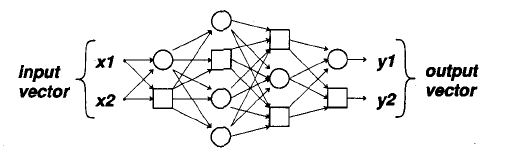
\includegraphics[width=\textwidth]{adaptive_net}
\caption {Arhitectura unei re'tele adaptive cu dou;a intr;ari 'si dou;a ie'siri}
\end{figure}
\newpage

\paragraph{}

A'sa cum am enun'tat 'inainte, o re'tea adaptiv;a este o re'tea multi-strat feedforward 'in care fiecare nod evalueaz;a o anumit;a func'tie (numit;a 'si func'tie de nod) pe semnalele de intrare, 'si, 'in plus, fiecare nod are 'si o mul'time de parametri. Formulele pentru func'tiile de nod pot varia de la nod la nod, iar alegerea lor depinde de func'tia pe care re'teaua trebuie s;a o modeleze. O particularitate important;a este c;a leg;aturile dintre noduri indic;a doar direc'tia pe care o parcurge semnalul;\ nu exist;a niciun fel de ponderi asociate leg;aturilor dintre noduri.
\par
Figura 7.1 ilustreaz;a o posibil;a configura'tie a unei re'tele cu doi parametri de intrare 'si doi parametri de ie'sire. Pentru a diferen'tia tipurile de noduri dintr-o re'tea adaptiv;a, sunt folosite noduri 'in forma rotund;a pentru a indica un nod fixat, ce nu prime'ste parametri, 'si noduri 'in forma p;atrat;a pentru a indica noduri adaptive, ce primesc parametri. Mul'timea parametrilor unei re'tele adaptive este reuniunea tuturor mul'timilor de parametri ale tuturor nodurilor adaptive. Pentru a ob'tine o modelare a unei func'tii dup;a intr;ari 'si ie'siri, ace'sti parametri sunt actualiza'ti folosind datele de antrenare 'si o regul;a de 'inv;a'tare bazat;a pe gradient prezentat;a 'in continuare.
\par
Fie o re'tea adaptiv;a cu $L$ straturi 'si cu al k-lea strat av'and $\#(k)$ noduri. Not;am al i-lea nod de pe stratul k cu $(k, i)$ 'si func'tia de nod cu $O_{i}^{k}$. Din moment ce semnalul de ie'sire al unui nod depinde de semnalele de intrare 'si de parametrii s;ai, avem
\begin{equation}
O_{i}^{k} = O_{i}^{k} (O_{1}^{k-1}, ... , O_{\#(k-1)}^{k-1}, a, b, c, ...)
\end{equation}
unde $a, b, c, ...$ sunt parametrii corespunz;atori acestui nod. (Not;a: am folosit $O_{i}^{k}$ at'at pentru a ne referi la semnalul de ie'sire al nodului c'at 'si la func'tia sa.)
\par
Av'and un set de date antrenare cu P intr;ari, putem defini m;asura de eroare pentru a $p$-a intrare ($1 \leq p \leq P$) din setul de date de antrenare ca fiind suma p;atratelor erorilor:
\begin{equation}
E_{p} = \displaystyle \sum_{m = 1}^{\#(L)} (T_{m, p} - O_{m, p}^{L})^{2}
\end{equation}
unde $T_{m, p}$ este a $m$-a component;a a celui de al $p$-lea vector 'tint;a de rezultate, iar $O_{m, p}^{L}$ este a $m$-a component;a a vectorului real de rezultate, produs prin prezentarea celui de-al $p$-lea vector de intr;ari.
\par
Prin urmare, m;asura total;a a erorii este
\begin{equation}
E = \displaystyle \sum_{p=1}^{P} E_{p}
\end{equation}

\paragraph{}
Pentru a ob'tine o procedur;a de 'inv;a'tare care s;a implementeze gradientul descendent 'in $E$ peste spa'tiul parametrilor, avem nevoie 'in primul r'and de rata de eroare $\frac {\partial E_{p}} {\partial O}$ pentru al $p$-lea punct din datele de antrenare 'si pentru fiecare ie'sire de nod $O$. Rata de eroare pentru nodul ($L, i$) devine (ob'tinut;a din 7.2)
\begin{equation}
\frac {\partial E_{p}} {\partial O_{i, p}^{k}} = -2(T_{i, p} - O_{i, p}^{L})
\end{equation}
Pentru nodul intern de la ($k, i$), rata de eroare poate fi derivat;a folosind regula 'inl;an'tuirii \footnote{Regula 'inl;an'tuirii este definit;a prin $\frac{dz}{dx} = \frac{dz}{dy} \cdot \frac{dy}{dx}$;\ i.e. av'and trei variabile $x, y, z$, cu $z$ dependent;a de $y$, iar $y$ dependent;a de $x$ astfel 'inc'at $y$ 'si $z$ sunt variabile dependente, atunci $z$, prin intermediul lui $y$ depinde de $x$.}
\begin{equation}
\frac {\partial E_{p}} {\partial O_{i, p}^{k}} = \displaystyle \sum_{m = 1}^{\#(k+1)} \frac {\partial E_{p}} {\partial O_{m, p}^{k+1}} \cdot \frac {\partial O_{m, p}^{k+1}} {\partial O_{i, p}^{k}}
\end{equation}
unde $1 \leq k \leq L-1$. Deci, rata de eroare a unui nod intern poate fi explicitat;a sub form;a de combina'tie liniar;a a ratelor de eroare ale nodurilor de pe stratul urm;ator. Prin urmare, pentru to'ti $1 \leq k \leq L$ 'si $1 \leq i \leq \#(k)$ putem g;asi $\frac {\partial E_{p}} {\partial O_{i, p}^{k}}$ conform cu 7.4 'si 7.5.
\par
S;a presupunem $\alpha$ un parametru al re'telei adaptive. Avem a'sadar
\begin{equation}
\frac {\partial E_{p}} {\partial \alpha} = \displaystyle \sum_{O^{*} \in S} \frac {\partial E_{p}} {\partial O^{*}} \cdot \frac {\partial O^{*}} {\partial \alpha}
\end{equation}
unde S este mul'timea nodurilor ale c;aror ie'siri depind de $\alpha$. Derivata m;asurii totale a erorii $E$ 'in raport cu $\alpha$ devine:
\begin{equation}
\frac {\partial E_{p}} {\partial \alpha} = \displaystyle \sum_{p = 1}^{P} \frac {\partial E_{p}} {\partial \alpha}
\end{equation}
\par
Formula de actualizare pentru parametrul generic $\alpha$ este:
\begin{equation}
\Delta \alpha = - \eta \frac {\partial E} {\partial \alpha}
\end{equation}
unde $\eta$ este rata de 'inv;a'tare care poate fi exprimat;a 'si ca:
\begin{equation}
\eta = - \frac {k} {\sqrt {\displaystyle \sum_{\alpha} \Big(\frac {\partial E} {\partial \alpha}\Big)^{2}}}
\end{equation}
unde $k$ este dimensiunea pasului, adic;a lungimea fiec;arei tranzi'tii a gradientului 'in spa'tiul parametrilor. De obicei, valorea lui $k$ poate fi schimbat;a pentru a varia viteza de convergen't;a.
\par
Exist;a dou;a metode de 'inv;a'tare pentru re'telele adaptive. Prin 'inv;a'tarea de tip batch (off-line) formula de actualizare a parametrului $\alpha$ este bazat;a pe (7.7), iar ac'tiunea de actualizare are loc doar atunci c'and intreg setul de date de antrenare a fost parcurs, i.e. dup;a o epoc;a.
\par
'In contrast, dac;a dorim ca parametrii s;a fie actualiza'ti imediat cum o pereche intrare-ie'sire i-a fost prezentat;a re'telei, atunci formula de 'inv;a'tare este bazat;a pe (7.6), 'si ne vom referi la ea ca 'inv;a'tare pattern (sau on-line). 'In continuare, prezent;am o derivare a unei reguli hibride 'si rapide sub ambele forme: off-line si on-line.
\par
\subsection{Regula de 'inv;a'tare hibrid;a off-line}
\paragraph{}

Regula de 'inv;a'tare hibrid;a off-line propune o combina'tie 'intre metoda gradientului 'si metod;a estim;arii p;atratelor minime pentru a identifica parametrii. De'si s-ar putea aplica metoda gradientului, aceasta este lent;a 'si exist;a posibilitatea ca ea s;a r;aman'a blocat;a 'in minime locale.
\par
S;a presupunem c;a re'teaua adaptiv;a pe care vom aplica regula are o singur;a ie'sire:
\begin{equation}
ie'sire = F(\overrightarrow{I}, S)
\end{equation}
unde $\overrightarrow{I}$ este mul'timea variabilelor de intrare 'si $S$ este mul'timea parametrilor. Dac;a exist;a o func'tie $H$ astfel 'inc'at compunerea $H \circ F$ este liniar;a 'in unele elemente din $S$, atunci aceste elemente pot fi identificate prin metoda p;atratelor minime. Formal, daca descompunem $S$ 'in
\begin{equation}
S = S_{1} \oplus S_{2}
\end{equation}
unde $\oplus$ reprezint;a 'insumarea direct;a, astfel 'inc'at $H \circ F$ este liniar;a 'in $S_{2}$, atunci aplic'and $H$ pe (7.10) avem
\begin{equation}
H(ie'sire) = H \circ F(\overrightarrow{I}, S)
\end{equation}
care este liniar;a 'in $S_{2}$. Date fiind valorile elementelor din $S_{1}$ putem introduce datele de antrenare $P$ 'in (7.12) ob'tin'and o ecua'tie matriceal;a:
\begin{equation}
AX = B
\end{equation}
unde $X$ este un vector de necunoscute ale c;arui elemente sunt parametri 'in $S_{2}$. Fie $|S_{2}| = M$, atunci dimensiunile lui $A, X$ 'si $B$ sunt $P \times M, M \times 1$, respectiv $P \times 1$. Din moment de $P$ este, de obicei, mai mare dec'at $M$ (num;arul de puncte de date de antrenare este mai mare dec'at num;arul de parametri liniari), aceasta este o problem;a compatibil nedeterminat;a, 'si, 'in general, nu exist;a o solu'tie exact;a pentru (7.13). Prin urmare, o estimare a celor mai mici p;atrate ale lui $X$, $X^{*}$, este c;autat;a pentru a minimiza eroarea p;atrat;a $||AX - B||^{2}$. Aceasta este o problem;a standard ce st;a la baza regresiei liniare, filtr;arii adaptive 'si proces;arii de semnale. Cea mai cunoscut;a formul;a pentru $X^{*}$ se folose'ste de pseudo-inversa lui $X$:
\begin{equation}
X^{*} = (A^{T}A)^{-1}A^{T}B
\end{equation}
unde $A^{T}$ este transpusa lui $A$, iar $(A^{T}A)^{-1}A^{T}$ este pseudo-transpusa lui $A$, dac;a $A$ este non-singular;a. De'si (7.14) are o nota'tie clar;a, 'si ea este u'sor de construit intuitiv, calcularea inversei este un proces foarte costisitor din punct de vedere computa'tional. Mai mult, ecua'tia nu este bine definit;a dac;a $A^{T}A$ este singular;a. Prin urmare, \cite{anfis} prezint;a o metod;a secven'tial;a de a calcula estimarea celor mai mici p;atrate ale lui $X$. Aceast;a metod;a secven'tial;a este eficient;a, 'si poate fi modificat;a 'intr-o variant;a on-line.
\par
Fie al $i$-lea vector r'and din matricea $A$ definit;a 'in (7.13) notat cu $a_{i}^{T}$, 'si al $i$-lea element din $B$ notat cu $b_{i}^{T}$. Atunci $X$ poate fi calculat iterativ folosind formule secven'tiale adoptate din literatur;a:
\begin{equation}
\begin{aligned}
X_{i+1} = X_{i} + S_{i+1}a_{i+1}(b_{i+1}^{T} - a_{i+1}^{T}X_{i}) \\
S_{i+1} = S_{i} - \frac {S_{i}a_{i+1}a_{i+1}^{T}S_{i}} {1 + a_{i+1}^{T}S_{i}a_{i+1}},\  i = 0, 1, ..., P-1
\end{aligned}
\end{equation}
unde $S_{i}$ este matricea de covarian't;a 'si estimarea celor mai mici p;atrate este egal;a cu $X_{P}$. Condi'tiile ini'tiale pentru a aplica \textit{bootstrapping}\footnote {Bootstrapping este o metod;a de inferen't;a statistic;a bazat;a pe folosirea unei singure e'santion;ari 'si 'inlocuirea  aleatorie a unor puncte din datele e'santionate cu alte puncte din acela'si e'santion, 'in mod repetat.} sunt $X_{0} = 0$ 'si $S_{0} = \gamma I$, unde $\gamma$ este un num;ar pozitiv mare, iar $I$ este matricea identitate de dimensiune $M \times M$.
Atunci c'and re'teaua adaptiv;a are mai multe ie;siri, ($ie'sire$ din (7.10) este un vector coloan;a), atunci (7.15) r;am'ane valabil;a, dar $b_{i}^{T}$ devine al $i$-lea r'and din $B$.
\par
Putem acum s;a combin;am metoda gradientului 'si metoda estim;arii p;atratelor minime pentru a actualiza parametrii dintr-o re'tea adaptiv;a. Fiecare epoc;a a acestei proceduri hibride de 'inv;a'tare este compus;a dintr-o propagare 'inainte 'si o propagare 'inapoi. 'In propagarea 'inainte oferim datele de intrare 'si semnalele func'tionale, iar acestea se propag;a 'inainte pentru a calcula ie'sirea fiec;arui nod p'an;a se ob'tin matricele $A$ 'si $B$ din (7.13), iar parametrii din $S_{2}$ sunt identifica'ti dup;a formula secven'tial;a a celor mai mici p;atrate din (7.15). Dup;a ce au fost identifica'ti parametrii din $S_{2}$, semnalele func'tionale continu;a s;a se propage 'inainte p'an;a c'and m;asura erorii este calculat;a. 'In propagarea 'inapoi ratele de eroare (derivatele m;asurii erorii 'in raport cu fiecare ie'sire de nod) se propag;a dinspre ie'siri c;atre intr;ari, iar parametrii din $S_{1}$ sunt actualiza'ti dup;a metoda gradientului din (7.9).
\par
Pentru valori fixate date parametrilor din $S_{1}$, este garantat c;a valorile parametrilor din $S_{2}$ sunt puncte globale de optim din spa'tiul parametrilor lui $S_{2}$ datorit;a alegerii m;asurii de eroare a p;atratelor. Nu numai c;a aceast;a regul;a hibrid;a de 'inv;a'tare descre'ste dimensiunea spa'tiului de c;autare din metoda gradientului, dar, 'in general, va avea un timp de convergen't;a substan'tial mai mic.
\par
Lu'and ca exemplu o re'tea neuronal;a cu propagare 'in spate 'si func'tia de activare sigmoid, dac;a ea are $p$ unit;a'ti de ie'sire, atunci $ie'sire$ din (7.10) este un vector coloan;a. Fie $H(\cdot)$ inversa func'tiei sigmoid:
\begin{equation}
H(x) = ln (\frac {x} {1-x})
\end{equation}
atunci (7.12) devine o func'tie liniar;a astfel 'inc'at fiecare element din $H(ie'sire)$ este o combina'tie liniar;a 'intre parametrii (ponderi 'si praguri) ce 'tin de stratul cu num;arul 2. 'In alte cuvinte, \\
$S_{1}$ =  ponderile 'si pragurile stratului ascuns \\
$S_{2}$ = ponderile 'si pragurile stratului de ie'sire \\
Prin urmare, putem aplica regula de 'inv;a'tare back-propagation pentru a regla parametrii stratului ascuns, 'si parametrii stratului de ie'sire pot fi identifica'ti de c;atre metoda celor mai mici p;atrate. Trebuie totu'si notat c;a folosind metoda celor mai mici p;atrate peste datele transformate de c;atre $H(\cdot)$ , parametrii ob'tinu'ti sunt optimi 'in func'tie de m;asura erorii cu eroarea la p;atrat, 'in loc de cea original;a. De obicei, acest lucru nu ridic;a o problem;a real;a c'at timp $H(\cdot)$ este monoton cresc;atoare.
\par

\subsection{Regula de 'inv;a'tare hibrid;a on-line}
\paragraph{}

Dac;a parametrii sunt actualiza'ti dup;a fiecare prezentare a datelorf atunci avem de a face cu paradigma 'inv;a'tarii on-line. Aceast;a paradigm;a este crucial;a pentru identificarea parametrilor 'in sistemele cu caracteristici care sunt 'in schimbare. Pentru a modifica regula off-line 'intr-o variant;a off-line este suficient s;a observ;am c;a gradientul descendent trebuie s;a fie bazat pe $E_{p}$ (vezi (7.6)) 'in loc de $E$. Formal, aceasta nu este o procedur;a 'in gradient adev;arat;a de minimizare a lui $E$, dar ea o va aproxima dac;a rata de 'inv;a'tare este mic;a.
\par
Pentru ca formula secven'tial;a a celor mai mici p;atrate s;a poat;a fi adaptat;a la caracteristicile variabile 'in func'tie de timp ale datelor de intrare, este necesar ca perechile de date vechi s;a aib;a o pondere din ce 'in ce mai mic;a odat;a ce apar date noi. 'Inc;a odat;a, aceast;a problem;a este studiat;a 'si rezolvat;a 'in literatura controlului adaptiv. O metod;a este formularea m;asurii erorii p;atratelor 'intr-o variant;a ponderat;a, unde datele mai vechi primesc factori mai mici de pondere fa't;a de cele mai noi. Acest lucru este echivalent cu ad;augarea unui factor de uitare $\lambda$ 'in formula secven'tial;a original;a:
\begin{equation}
\begin{aligned}
X_{i+1} = X_{i} + S_{i+1}a_{i+1}(b_{i+1}^{T} - a_{i+1}^{T}X_{i}) \\
S_{i+1} = \frac {1}{\lambda} [S_{i} - \frac {S_{i}a_{i+1}a_{i+1}^{T}S_{i}} {\lambda + a_{i+1}^{T}S_{i}a_{i+1}}],\  i = 0, 1, ..., P-1
\end{aligned}
\end{equation}
unde $\lambda$ este 'intre $0$ 'si $1$. Cu c'at $\lambda$ descre'ste, cu at'at mai mult se observ;a efectele sl;abirii datelor vechi. Dar, uneori, un $\lambda$ mic poate duce la instabilitate numeric;a, deci ar trebui evitat.

\newpage
\subsection{Arhitectura ANFIS}
\paragraph{}

'Stiind acum defini'tia, arhitectura 'si regulile de 'inv;a'tare ale unei re'tele adaptive, putem deduce faptul c;a func'tional, nu exist;a aproape nicio constr'angere asupra func'tiilor de nod 'in afar;a de diferen'tiabilitatea pe por'tiuni\footnote{O func'tie $f$ se nume'ste diferen'tiabil;a pe por'tiuni dac;a: \\
$f$ este definit;a pe por'tiuni (exist;a mai multe sub-func'tii ale lui $f$, fiecare aplicat;a pentru un anumit interval din domeniul lui $f$) \\
Pentru fiecare por'tiune a lui $f$, subfunc'tia corespunz;atoare acelei por'tiuni este diferen'tiabil;a de-a lungul 'intregului subdomeniu}, iar structural, singura limitare a configura'tiei re'telei este c;a aceasta trebuie sa fie de tip feedforward. Datorit;a acestor restric'tii minimale, observ;am c;a aplica'tiile re'telelor adaptive sunt vaste 'si imediate 'in diverse domenii. Vom prezenta 'in continuare o arhitectur;a de re'tele care sunt echivalente func'tional cu un sistem de inferen't;a fuzzy. Vom descrie o metod;a de descompunere a mul'timii parametrilor pentru a aplica regula de 'inv;a'tare hibrid;a.
\par
S;a presupunem un sistem de inferen't;a fuzzy cu dou'a variabile de intrare $x, y$ 'si una de ie'sire $z$. Presupunem c;a baza de reguli con'tine dou'a reguli fuzzy if-then de tip Takagi-Sugeno:
\begin{enumerate}
\item if $x$ is $A_{1}$ and $y$ is $B_{1}$ then $f_{1} = p_{1}x + q_{1}y + r_{1}$
\item if $x$ is $A_{2}$ and $y$ is $B_{2}$ then $f_{2} = p_{2}x + q_{2}y + r_{2}$
\end{enumerate}
\begin{figure}[!htbp]
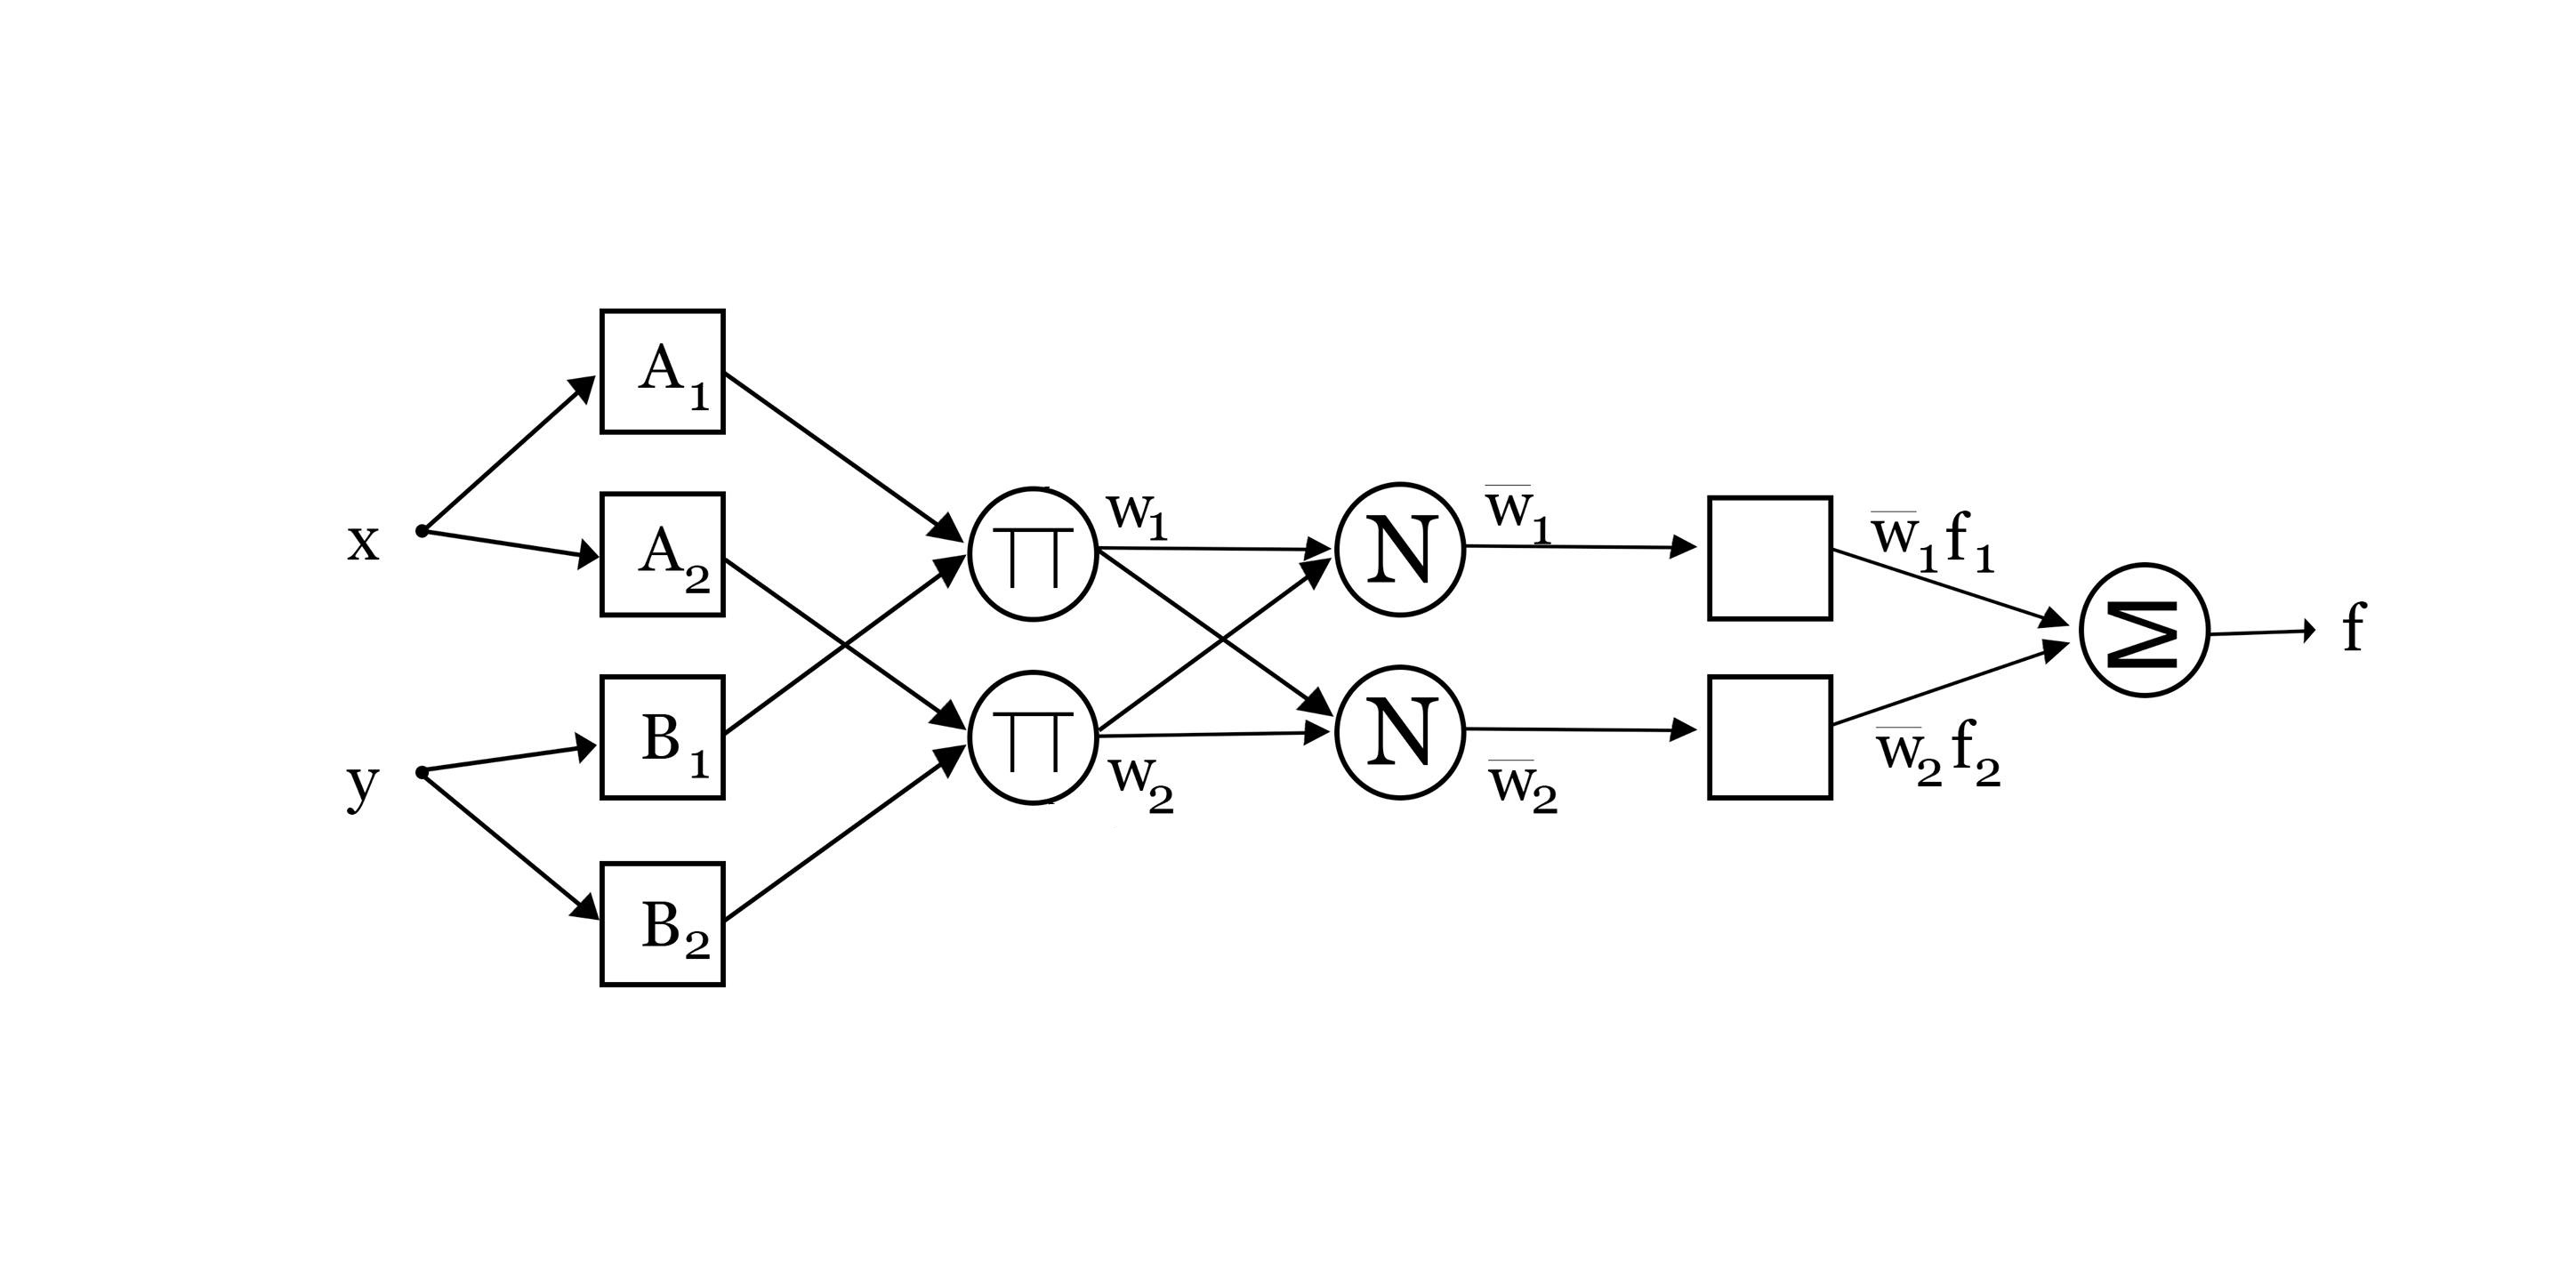
\includegraphics[width=\textwidth]{anfisarch}
\caption{Arhitectur;a ANFIS pentru dou;a reguli fuzzy if-then Takagi-Sugeno.}
\end{figure}
\newpage
\paragraph{}
Toate func'tiile de node apar'tin uneia din familiile de func'tii definite 'in continuare, 'in func'tie de strat:
\begin{enumerate}
\item [Stratul 1:] Fiecare nod $i$ din acest strat este un nod adaptiv cu o func'tie de nod 
\begin {equation}
O_{i}^{1} = \mu_{A_{i}}(x)
\end{equation}
unde $x$ este intrarea pentru nodul $i$, 'si $A_{i}$ este eticheta 'in limbaj natural (i.e. mic, mare, etc.) asociat;a acestei func'tii de nod. Altfel spus, $O_{i}^{1}$ este func'tia de apartenen't;a a lui $A_{i}$, specific'and gradul cu care un $x$ dat satisface cuantificatorul $A_{i}$. De obicei, se alege $\mu_{A_{i}}(x)$ astfel 'inc'at s;a fie gaussian;a cu maximul egal cu $1$ 'si minimul egal cu $0$, cu formele:
\begin{equation}
\mu_{A_{i}}(x) = \frac {1} {1 + [(\frac {x - c_{i}} {a_{i}})^2]b_{i}}
\end{equation}
sau
\begin{equation}
\mu_{A_{i}}(x) = exp[- (\frac {x-c_{i}} {a_{i}} )^{2}]
\end{equation}
unde \{$a_{i}, b_{i}, c_{i}$\} este mul'timea de parametri. 'In func'tie de schimb;arile parametrilor, func'tiile gaussiene variaz;a corespunz;ator, ar;at'and astfel diefirte forme de func'tii de apartenen't;a peste eticheta 'in limbaj natural $A_{i}$. De fapt, orice func'tii continue 'si diferen'tiabile pe por'tiuni, cum ar fi func'tiile de apartenen't;a trapezoidale sau triunghiulare, sunt candida'ti buni pentru acest strat. Parametrii acestui strat se mai numesc 'si parametri de premise.
\item [Stratul 2:] Fiecare nod din acest strat este un nod fix (i.e. nu are parametri) etichetat cu $\Pi$, care 'inmul'te'ste semnalele primite 'si trimite produsul acestora. De exemplu,
\begin{equation}
w_{i} = \mu_{A_{i}}(x) \times \mu_{B_{i}}(y),\ i = 1,2.
\end{equation}
Fiecare ie'sire de nod reprezint;a puterea de "aprindere" a regulii. Mai mult, orice al'ti operatori T-norma'ti care calculeaz;a un "'SI" generalizat pot fi folosite ca func'tii de nod pe acest strat.
\item [Stratul 3:] Fiecare nod de pe acest strat este un nod fix etichetat cu "N". Cel de-al $i$-lea nod calculeaz;a raportul puterii de "aprindere" a celei de a $i$-a regul;a la suma tuturor puterilor de "aprindere" ale regulilor.
\begin{equation}
\bar w_{i} = \frac {w_{i}} {w_{1} + w_{2}},\ i = 1, 2
\end{equation}
Ie'sirile acestui strat se mai numesc 'si puterile de "aprindere" normalizate.
\item [Stratul 4:] Fiecare nod $i$ din acest strat este un nod adaptiv, cu func'tia
\begin{equation}
O_{i}^{4} = \bar w_{i}f_{i} = \bar w_{i} (p_{i}x + q_{i}y + r_{i})
\end{equation}
unde $\bar w_{i}$ este ie'sirea stratului $3$, iar $\{p_{i}, q_{i}, r_{i}\}$ este mul'timea parametrilor. Parametrii acestui strat se mai numesc 'si parametrii consecven'ti.
\item [Stratul 5:] Singurul nod din acest strat este un nod fix etichetat cu $\sigma$ care calculeaz;a semnalul general de ie'sire ca fiind suma tuturor semnalelor care ajung la el
\begin{equation}
O_{1}^{5} = \text{ie'sire general;a} = \displaystyle \sum_{i} \bar w_{i}f_{i} = \frac {\sum_{i} w_{i}f_{i}} {\sum_{i} w_{i}}
\end{equation}
\end{enumerate}
\par

Av'and toate straturile definite ob'tinem construc'tia unei re'tele adaptive ce modeleaz;a un sistem de inferen't;a fuzzy format din reguli if-then de tipul Takagi-Sugeno. 

\subsection{Aplicarea algoritmului de 'inv;a'tare hibrid}

Continu'and cu acela'si exemplu ca 'in sec'tiunea 7.5, avem un sistem de inferen't;a fuzzy cu dou;a reguli:
\begin{equation}
\begin{aligned}
f_{1} = p_{1}x + q_{1}y + r_{1} \\
f_{2} = p_{2}x + q_{2}y + r_{2}
\end{aligned}
\end{equation}
Se poate observa c;a dac;a avem valorile parametrilor de premise, putem exprima ie'sirea final;a sub form;a de combina'tie liniar;a a parametrilor consecven'ti. Mai precis, putem scrie ie'sirea $f$ ca:
\begin{equation}
\begin{aligned}
f = \frac {w_{1}} {w_{1} + w_{2}} f_{1} + \frac {w_{2}} {w_{1} + w_{2}} f_{2} \\
  = \bar w_{1}f_{1} + \bar w_{2} + f_{2} \\
  = (\bar w_{1}x)p_{1} + (\bar w_{1}y)q_{1} + (\bar w_{1})r_{1} + \\(\bar w_{2}x)p_{2} + (\bar w_{2}y)q_{2} + (\bar w_{2})r_{2}
\end{aligned}
\end{equation}
Observ;am c;a $f$ este liniar;a 'in parametrii consecven'ti $p_{1}, q_{1}, r_{1}, p_{2}, q_{2}, r_{2}$. Ob'tinem
\begin{equation}
S = S_{1} \cup S_{2}
\end{equation}
unde $S$ = mul'timea tuturor parametrilor, $S_{1}$ = mul'timea parametrilor de premise 'si $S_{2}$ = mul'timea parametrilor consecven'ti pentru ecua'tia (7.11). $H(\cdot)$ 'si $F(\cdot, \cdot)$ sunt func'tiile identitate, respectiv func'tia sistemului de inferen't;a fuzzy. Prin urmare, regula de 'inv;a'tare hibrid;a poate fi aplicat;a direct;\ 'in direc'tia 'inainte a regulii semnalele func'tiilor ajung p'an;a 'in stratul 4, iar parametrii consecven'ti sunt identifica'ti de estimarea celor mai mici p;atrate. 'In direc'tia 'inapoi, ratele de eroare se propag;a 'inapoi, iar parametrii de premise sunt actualiza'ti dup;a regula gradientului descendent.














\section {M;asura performan'tei modelelor}
\subsection{Root mean squared error - RMSE}

\paragraph{}
RMSE este des folosit;a 'si este o metric;a general;a de erori pentru predic'tiile numerice. Comparat;a cu alte metrici, cum ar fi cea a mediei absolute a erorilor, RMSE amplific;a 'si scoate 'in eviden't;a toate erorile mari.
\par
Formula pentru RMSE este:
\begin{equation}
RMSE = \sqrt{\frac {1} {n} \displaystyle \sum_{i=1}^{n}(y_i -\hat  y_i)^2}
\end{equation}

\subsection{Mean Magnitude Relative Error - MMRE}
\paragraph{}
Metrica MMRE este una dintre cele mai folosite 'in interpretarea acurate'tei unui model estimativ de cost. 
Pentru a ajunge la calculul MMRE este nevoie ca ini'tial s;a fie calculat;a pentru fiecare punct din date metrica MRE (mean relative error), cu formula
\begin{equation}
MRE_i = \frac {|y_i - \hat y_i|} {y_i}
\end{equation}
Av'and MRE calculat pentru toate punctele, MMRE este definit ca
\begin{equation}
MMRE = \frac {1} {N} \displaystyle \sum_{i=1}^{N}MRE_i
\end{equation}
\subsection{PRED(25)}
\paragraph{}
PRED(25) este o alt;a metric;a utilizat;a pentru a interpreta acurate'tea unui model estimativ de cost. Aceast;a m;asoar;a c'ate din estim;arile f;acute se 'incadreaz;a 'intr-o rat;a de +/- 25\% fa't;a de valorea real;a.
\begin{equation}
PRED(25) = \frac{1} {N} \displaystyle \sum_{i=1}^{N} \begin {cases} 1 \quad \text{dac;a $MRE_i \leq x$} \\
										       0 \quad \text {altfel}
							 	\end{cases}
\end{equation}
\section {Rezultate experimentale}

\paragraph{}
Av'and definite re'telele de tip ANFIS 'si cunosc'and acum modelul COCOMO, reamintim scopul experimentului: predic'tia efortului dezvolt;arii unui proiect software plec'and de la factorii de cost COCOMO 'si estimarea proiectului 'in mii de linii de cod surs;a livrate. 
\par
\subsection{Metodologia de lucru}
Datele pe care le-am folosit au fost prezentate 'in capitolul 4. Acestea au fost 'imp;ar'tite, 'in mod randomizat, 'in 85\% date de antrenare 'si 15\% date de testare. Urm;atorul pas a fost aplicarea normaliz;arii min-max peste acestea, astfel 'inc'at valorile extreme s;a nu aib;a o pondere exagerat;a fa't;a de restul datelor.
\begin{figure}[!htbp]
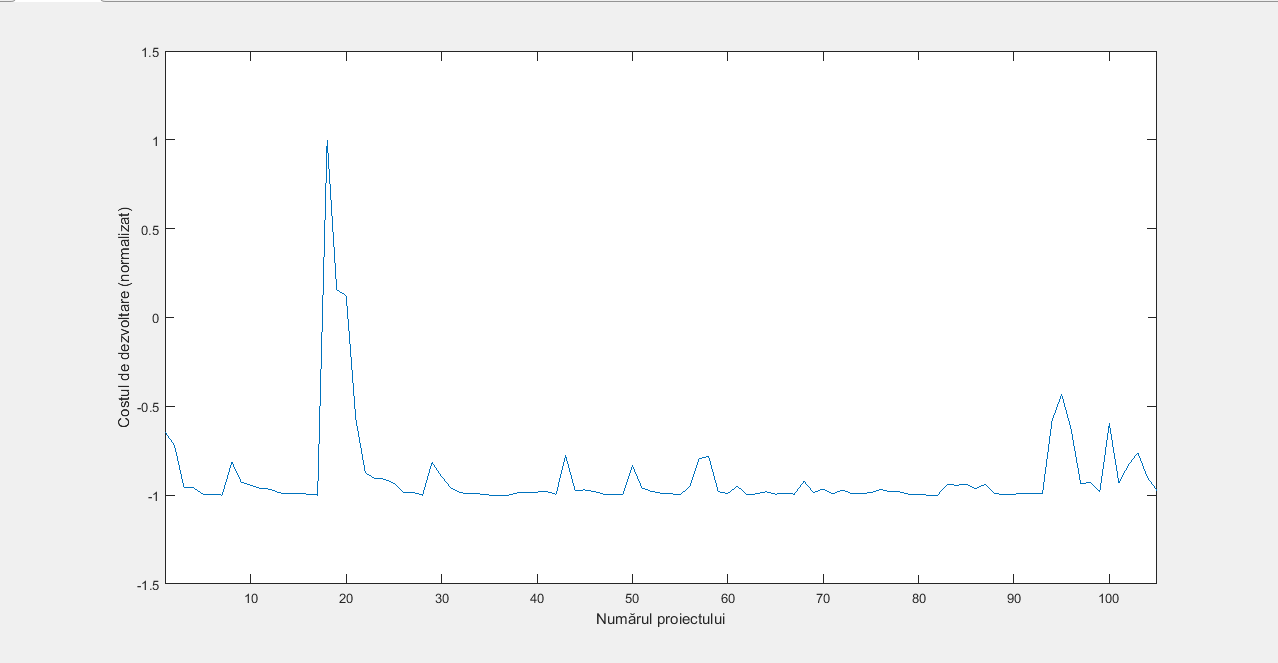
\includegraphics[width=\textwidth]{training_cost}
\caption{Reparti'tia costurilor din mul'timea de antrenare pentru fiecare proiect}
\end{figure}
\par
Putem observa u'sor din Figura 9.1 c;a exist;a valori extreme 'in date, astfel justific'and normalizarea datelor.
\par
Odat;a normalizate datele am creat un sistem de inferen't;a fuzzy pentru datele de intrare, folosind algoritmul de clustering subtractiv, cu valorile 0.8 pentru "Cluster Influence Range", 0.4 pentru "Squash Factor", 0.2 pentru "Accept Ratio" 'si 0.07 pentru "Reject Ratio". Astfel s-a ob'tinut un sistem de inferen't;a fuzzy cu 64 de clustere, fiecare cu c'ate 16 reguli de apartenen't;a pe antecedent.
\par
Sistemul de inferen't;a fuzzy a fost antrenat folosind algoritmul ANFIS pentru 100 de epoci, astfel ajung'and s;a ob'tin;a o eroare RMSE de 'inv;a'tare de 0.0008. Eroarea MMRE este de 0.000270 peste mul'timea de antrenare. Rezultatele pot fi vizualizate 'in figura 9.2.
\newpage
\begin{figure}[!htbp]
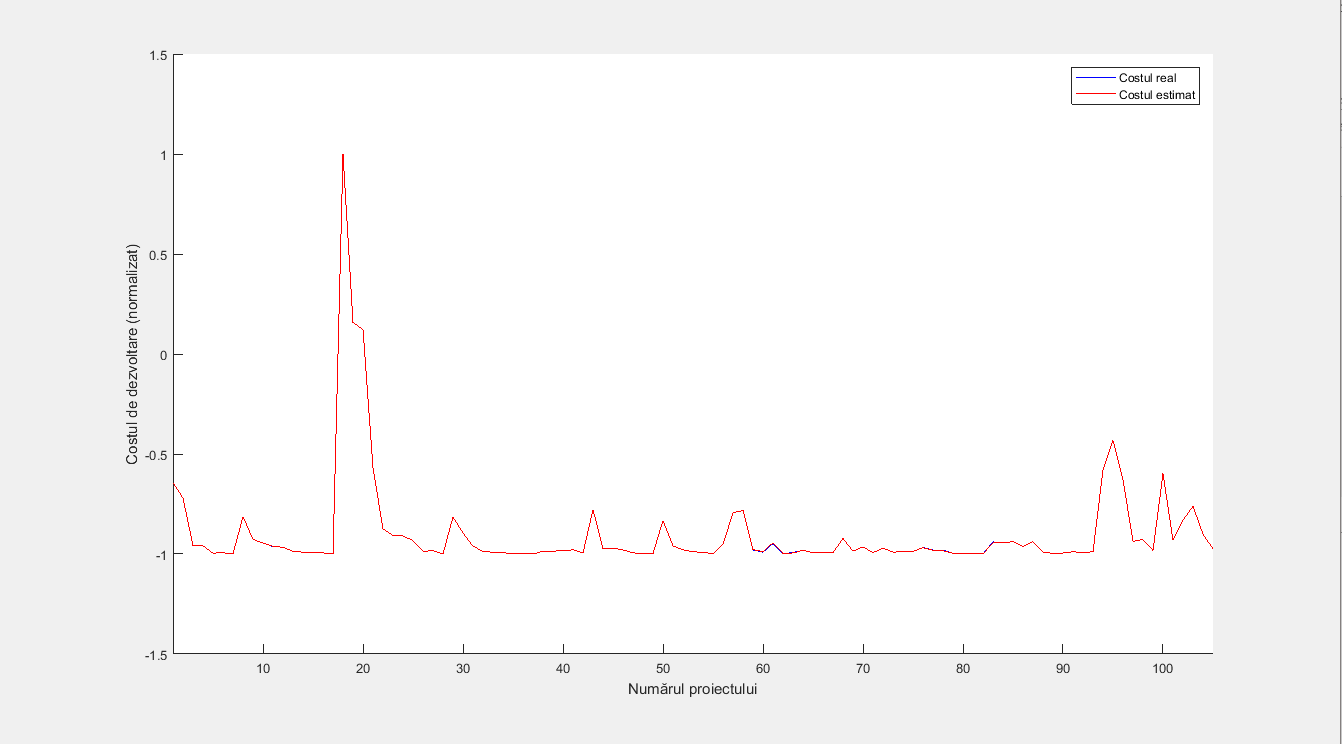
\includegraphics[width=\textwidth]{training_estimated}
\caption{Rezultatele antren;arii vs valorile reale}
\end{figure}
\par
Putem observa o 'inv;a'tare aproape complet;a a datelor de antrenare. Acest lucru nu este neap;arat dezirabil, fiind un indicator c;a modelul sufer;a de overfitting. Ne vom pronun;ta asupra acestui lucru dup;a observarea comportamentului peste datele de testare.
\subsection{Rezultatele evalu;arii re'telei}
P;astr'and re'teaua antrenat;a mai devreme, o vom supune simul;arii peste cele 18 puncte de test pe care le avem la dispozi'tie. 
\par
Rezultatele evalu;arii sunt urm'atoarele:
\begin{itemize}
\item O eroare RMSE de 0.059
\item O eroare MMRE de 0.036
\item O estimare PRED(25) de 1
\end{itemize}
Astfel, este evident c;a fenomenul de overfitting nu a avut loc, sau dac;a acesta a ap;arut se manifest;a insesizabil. Prin urmare, consider;am c;a modelul propus ne ofer;a o rat;a de 'inv;a'tare foarte bun;a, fiind capabil s;a ofere predic'tii cu acurate'te foarte bun;a pentru proiectele modelate sub COCOMO.
\newpage
\begin{figure}[!htbp]
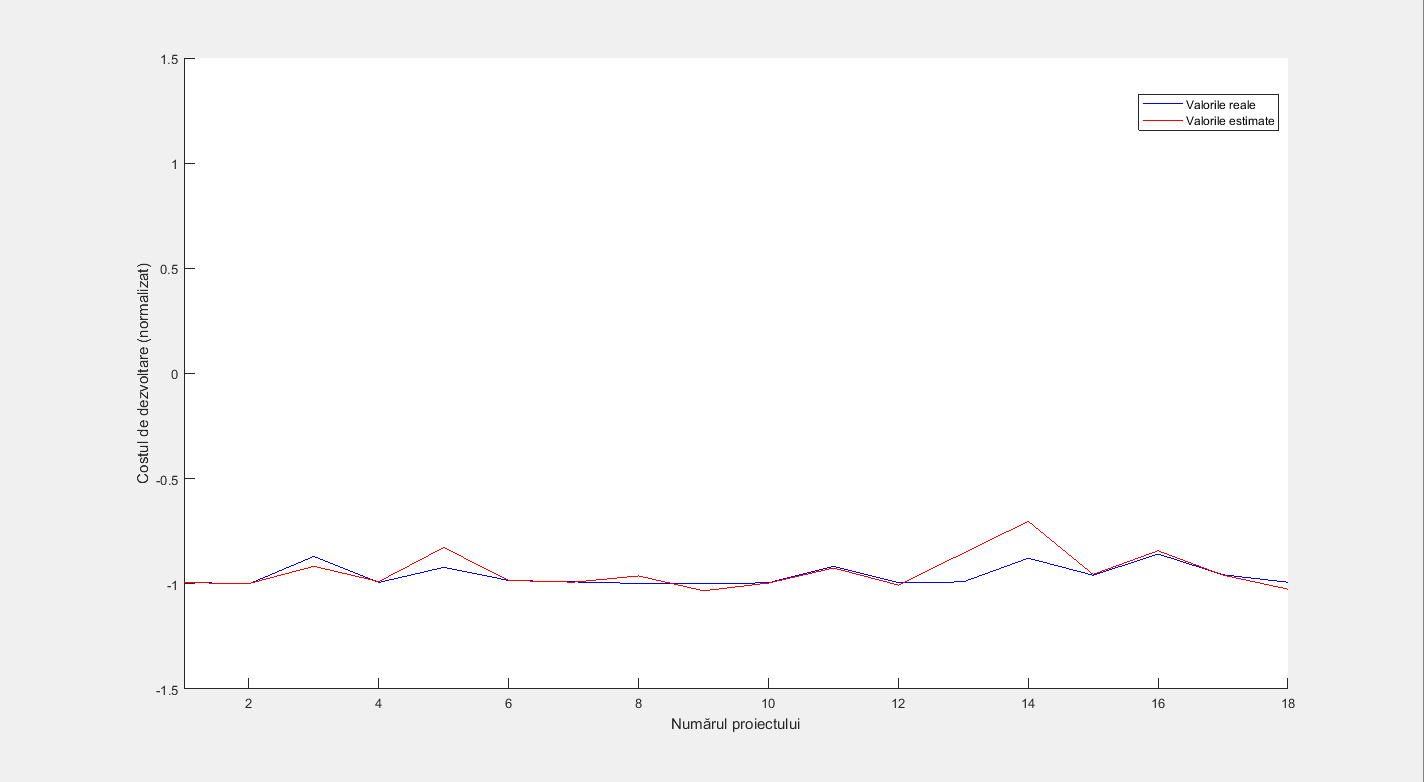
\includegraphics[width=\textwidth]{testing_output}
\caption {Rezultatele evalu;arii datelor de test vs valorile reale}
\end{figure}
\section{Rezultatele modelului cu re'tele neuronale}

\subsection{Metodologia de lucru}
\paragraph{}
Am folosit acelea'si date ca 'si 'in capitolul 9, 'imp;ar'tite 'in 85\% date de antrenare, 'si 15\% date de testare. La fel ca 'inainte, am aplicat aceea'si normalizare min-max asupra lor 'inainte de a 'incepe antrenarea re'telei.
\par
Re'teaua a fost antrenat;a folosind algoritmul Levenberg-Marquardt de backpropagare, cu un strat ascuns de 10 perceptroni 'si un num;ar maxim de 1000 de epoci. Arhitectura re'telei poate fi observat;a 'in figura 10.1.
\begin{figure}[!htbp]
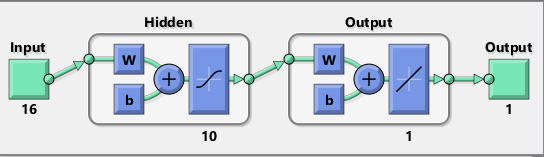
\includegraphics[width=\textwidth]{nnarch}
\caption {Arhitectura re'telei neuronale propuse}
\end{figure}
\subsection{Rezultatele evalu;arii re'telei}
\paragraph{}
Simularea peste cele 18 puncte de test au oferit urm;atoarele rezultate: 
\begin{itemize}
\item O eroare RMSE de 0.227
\item O eroare MMRE de 0.146
\item O estimare PRED(25) de 0.83
\end{itemize}
\par
\begin{figure}[!htbp]
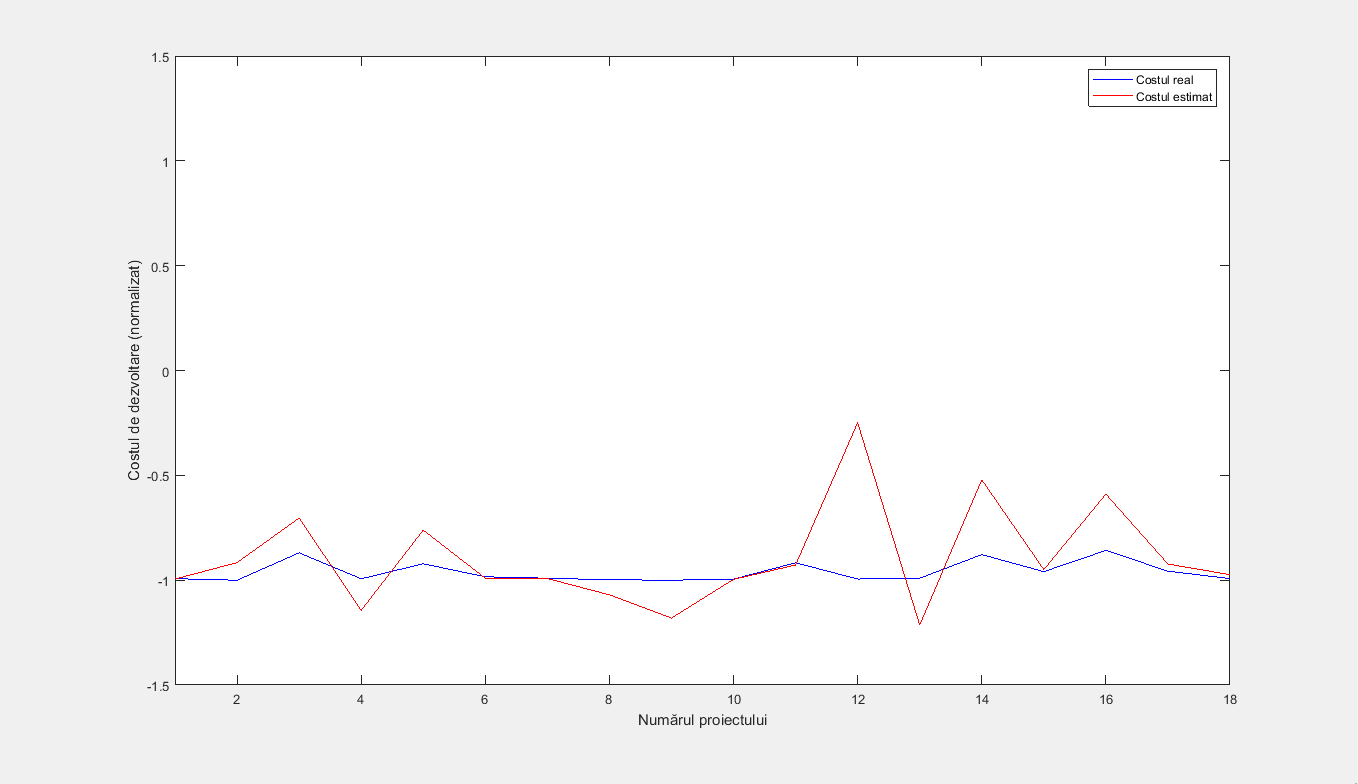
\includegraphics[width=\textwidth]{nntestoutput}
\caption{Rezultatele evalu;arii datelor de test folosind re'teaua neuronal;a propus;a}
\end{figure}
\par
Figura 10.2 ne ofer;a o viziune asupra felului 'in care re'teaua construie'ste predic'tiile peste datele de test. Putem observa c;a unele puncte sunt prezise cu o eroare semnificativ;a, lucru par'tial datorat unui set de date de antrenare restr'ans.
\section{Compararea rezultatelor}

\paragraph{}

Observ'and rezultatele ob'tinute prin evaluarea celor dou;a modele, observ;am c;a modelul bazat pe ANFIS ob'tine rezultate mai bune dec'at cel bazat pe re'tele neuronale prin toate metricile. Acest lucru este par'tial datorat faptului c;a ANFIS este construit astfel 'inc'at s;a ob'tin;a rezultate robuste peste date cu o oarecare incertitudine.
\par
Un alt motiv pentru care 'in acest experiment ANFIS ob'tine erori mai mici este acela c;a nu au existat suficiente date de antrenare 'si testare, acesta fiind un punct slab pentru re'telele neuronale, care au un sistem de inferen't;a foarte puternic atunci c'and li se pot prezenta baze de date cu un num;ar de intr;ari cu cel pu'tin un ordin de magnitudine mai mare dec'at am avut disponibile pentru acest studiu.
\begin{figure}[!htbp]
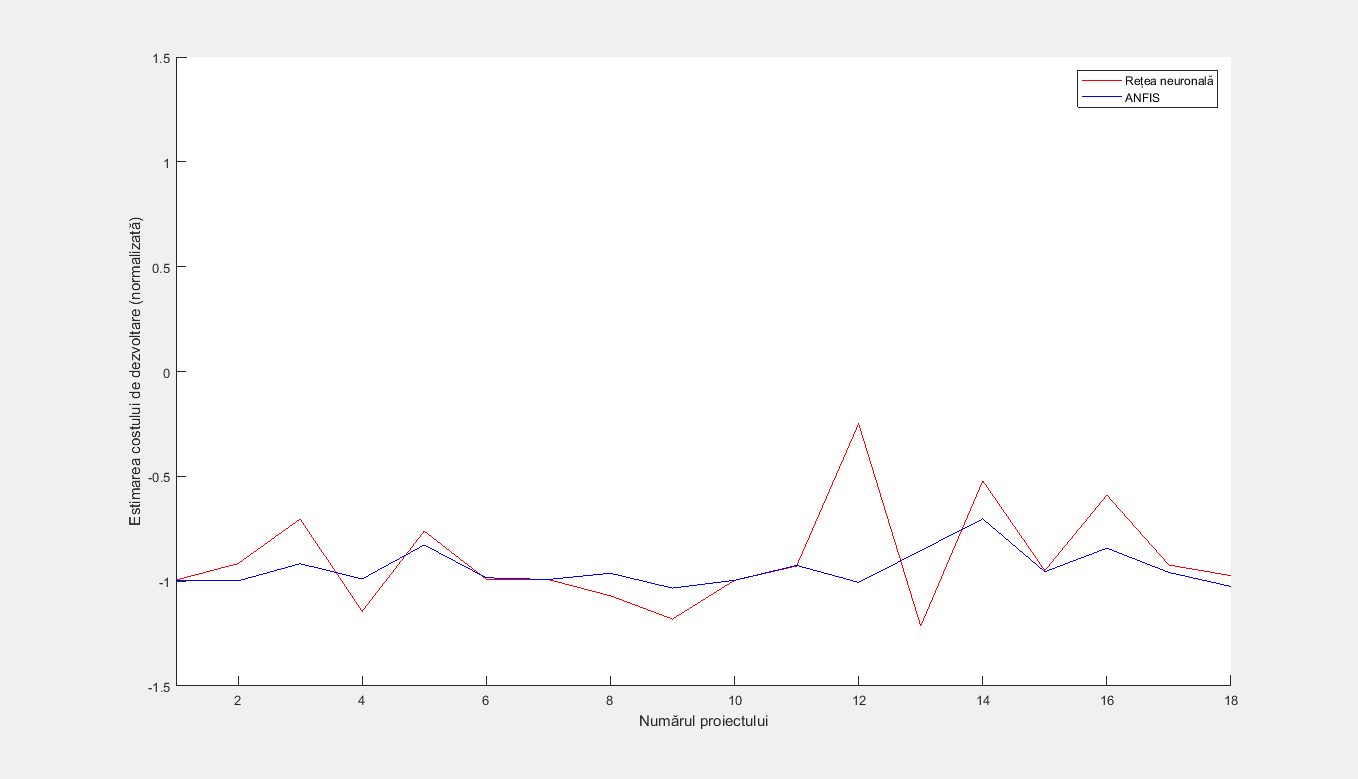
\includegraphics[width=\textwidth]{comparison}
\caption{ANFIS vs re'teaua neuronal;a peste datele de test}
\end{figure}
\par
Din figura 11.1 putem observa faptul c;a 'in afar;a de proiectele 12 'si 13, unde re'teaua neuronal;a ofer;a o estimare complet diferit;a fa't;a de ANFIS, 'in general, re'teaua neuronal;a urmeaz;a trendul ANFIS dar mult mai exagerat, 'intocmai datorit;a unor ponderi prea mari.
\section{Concluzii}
\paragraph{}

Aceast;a lucrare a fost o prezentare a unui model de re'tele neuro-fuzzy, 'si anume ANFIS, c'at 'si aplicarea acestuia asupra unui set de date bazat pe COCOMO. Pentru a ob'tine o viziune mai bun;a asupra performan'telor acestui model, rezultatele acestuia au fost comparate cu cele ob'tinute dintr-o re'tea neuronal;a clasic;a, fiind un model cunoscut 'si bine studiat.
\par
Rezultatele ini'tiale ne arat;a faptul c;a ANFIS se descurc;a foarte bine, cel pu'tin pentru acest set de date, ob'tin'and o predic'tie cu eroare sub 25\% pentru toate proiectele repartizate 'in mul'timea de testare. 'In cealalt;a parte, modelul bazat pe re'tele neuronale ob'tine aceea'si predic'tie doar 'in propor'tie de 83\%, fiind aproape la limita de a fi un predictor acceptabil.
\par
Consider;am c;a unul dintre cele mai puternice puncte ale acestei lucr;ari a fost 'inv;a'tarea peste toate cele 16 caracteristici ale modelului COCOMO, fa't;a de alte articole din literatur;a care se restr'ang la un num;ar mai mic de caracteristici. 'In plus, ANFIS poate fi 'in mod manual ajustat cu cuno'stin'te expert, fiind p'an;a la urm;a un sistem de inferen't;a fuzzy. Acest lucru permite 'si analizarea foarte u'soar;a 'in cazul 'in care estim;arile au erori foarte mari, fiind posibil;a g;asirea regulii 'si/sau a clusterului care genereaz;a aceste defecte.
\par
O viitoare direc'tie de cercetare poate consta 'in a g;asi metode c'at mai eficiente de integrare a cuno'stin'telor expert 'inc;a din momentul antren;arii re'telelor ANFIS, astfel 'imbun;at;a'tind eficien;ta 'inv;a'tarii. 'In plus, compara'tia ar putea fi reluat;a 'si 'imbun;at;a'tit;a at'at pentru re'telele ANFIS, c'at 'si pentru cele neuronale dac;a ar exista o metod;a verosimil;a de a genera mul'timi noi de proiecte sintetice sub modelul COCOMO.
\par
'In concluzie, noi consider;am modelul ANFIS ca av'and un domeniu de aplica'tie foarte bun 'in predic'tia efortului de dezvoltare ale proiectelor software. 'In plus, p;astr'and aceea'si arhitectur;a a re'telei, scopul acesteia poate fi schimbat pentru a prezice viitoarele defecte dintr-un proiect software (desigur, date fiind datele de antrenare corespunz;atoare) sau puncte 'in seriile de timp. Aplicabilitatea ANFIS a fost deja extins;a cu succes 'si in domeniul controlului automat, 'si cu siguran't;a acesta este doar 'inceputul.




\begin{thebibliography}{9}
\addcontentsline{toc}{section}{Bibliografie}
\bibitem{boehm}
Boehm, Barry W. (1981). \textit{Software Engineering Economics.} Prentice-Hall. 
\bibitem{anfis}
Jang, J.-S.R. (1993) ANFIS: Adaptive-Network-Based Fuzzy Inference System. \textit{IEEE Transactions On Systems, Man, And Cybernetics}, 23(3), pp. 665-685.
\bibitem{cocomoneuralnets}
Kaushik, A. et al. (2012) COCOMO Estimates Using Neural Networks \textit{I.J. Intelligent Systems and Applications}, 9, pp. 22-8.
\bibitem{anfiscost}
Mokri, F. D. et al. (2016) Software Cost Estimation using Adaptive Neuro Fuzzy Inference System \textit{International Journal of Academic Research in Computer Engineering}, 1(1), pp. 34-39.
\bibitem{promise1}
Promise Software Engineering Repository (2004), \textit{COCOMO Nasa/Software Cost Estimation}. [online] Disponibil la http://promise.site.uottawa.ca/SERepository/datasets/cocomonasa\_v1.arff (30 Aug. 2017)
\bibitem{promise2}
Promise Software Engineering Repository (2004), \textit{COCOMO 81/Software Cost Estimation}. [online] Disponibil la http://promise.site.uottawa.ca/SERepository/datasets/cocomo81.arff (30 Aug. 2017)
\bibitem{klirfuzzy}
Klir, George J. et al. (1995). \textit{Fuzzy Sets and Fuzzy Logic}. Pretince-Hall.
\bibitem{takagisugeno}
Takagi, T. et al. (1983) Derivation of fuzzy control rules from human operator's control actions. \textit{Proc. IFAC Symp. Fuzzy Inform., Knowledge Representation and Decision Analysis}, pp. 55-60.
\bibitem{fcmcluster}
Dunn, J. (1974). A fuzzy relative of the ISODATA process and its use in detecting compact, well separated cluster. \textit{J. Cybernetics}, 3(3), pp. 32-57.
\bibitem{subclustering}
Chiu, S. (1994). Fuzzy Model Identification Based on Cluster Estimation. \textit{Journal of the Intelligent and Fuzzy Systems}, 1(2), pp. 267-278.
\bibitem{statlearn}
Enachescu, D. (2003) \textit{Elements of Statistical Learning. Applications in Data Mining.} Cooperativa Libraria Editrice Universita di Padova.
\end{thebibliography}
\section{Anex;a}

\paragraph{}

Sursele folosite pentru aceast;a lucrare, seturile de date 'si documenta'tia \LaTeX\ pot fi g;asite la adresa https://github.com/nfmadar/finalver-unibuc2017 .
\newpage
\thispagestyle{empty}
\mbox{}
\newpage
\end{document}